\chapter{Irradiation Tests}
\label{chap:II-5-irradiation}

  The OptoHybrid will be located in a region of CMS exposed to fluxes of particles up to 20 kHz cm$^{-2}$, some of which might interact with the FPGA and cause errors in the logic. Those could in turn influence the functioning of the system and degrade its performance. To understand and potentially solve this issue, irradiation tests have been performed to measure the interaction cross section of the particles with the various components of the FPGA. Two OptoHybrids v2a programmed with a dedicated firmware designed to detect errors have been placed in a high intensity proton beam of fluxes up to 2 $ \times $ 10$^8$ particles cm$^{-2}$ s$^{-1}$. The two boards were each controlled by an additional OptoHybrid placed outside the test area which recorded the events and statistics. \\

  In this chapter, we provide the reader with an overview of the internal architecture of an FPGA to better understand the potential sources of errors and the effects of radiation. We then describe the firmware of the irradiated and control FPGAs which has been used during the test. The setup and beam parameters of the irradiation test are reviewed before presenting the results that were obtained after analysis.

  \section{Architecture of an FPGA}

    To optimize the occupancy of the resources of the FPGA and develop code that uses the full potential of the device, a deep comprehension of the intrinsic architecture of the chip is required. Although families of FPGAs differ in size and complexity, their building blocks remain the same and are described hereafter.

    \subsection{Configurable Logic Blocks (CLB)}

      Configurable Logic Blocks (CLBs) \cite{VIRTEX-CLB} are the building blocks of the FPGA used to implement sequential and combinatorial logic. They are composed of two important objects: Look-Up Tables (LUTs) and registers. LUTs are components which outputs are a function of the inputs as defined in a programmable table. They implement a truth table for every possible combination of the inputs which defines the value of the outputs. The response of a LUT to a change in the inputs is almost instantaneous. LUTs in the Xilinx Virtex-6 FPGAs can either implement functions with six inputs and a single output or functions with five inputs and two outputs. The outputs of the LUTs can, if so required by the design, be connected to registers which sample the signals at the rising edge of a given clock. Registers are used for their sample-and-hold functionality which makes designs synchronous to clocks. With these two components, CLBs can implement complex functions and describe intricate systems. \\

      \begin{figure}[p!]
        \centering
        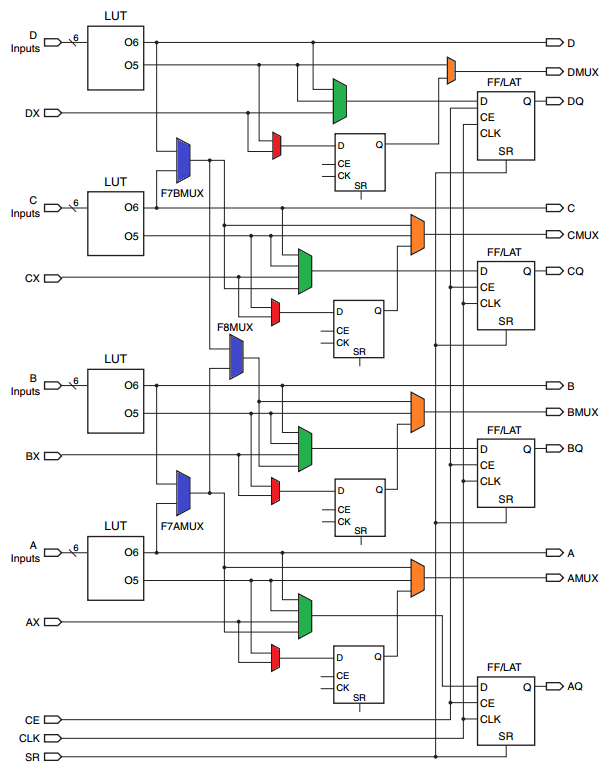
\includegraphics[width=\textwidth]{img/II-5-irradiation/clb.png}
        \caption{Simplified view of a slice composed of four LUTs on the left and eight registers on the right \cite{VIRTEX-CLB}.}
        \label{fig:II-5-clb}
      \end{figure}

      Each CLB is composed of two slices each made of four LUTs and eight registers which layout is shown in Figure \ref{fig:II-5-clb}. Each LUT is connected to an input bus of six signals (A, B, C, and D input buses) and to an unbuffered output bus of a single bit (O6 to A, B, C, and D). Four additional signals enter the slice (AX, BX, CX, and DX) and are connected to multiplexers (red) which allow to buffer either the former or the second output of the LUTs (O5). The output of the same buffer is then connected to a second multiplexer (orange) which allows to select either the former or an unbuffered output of the LUTs (AMUX, BMUX, CMUX, and DMUX). Finally, a third multiplexer (green) connects a range of signals to the registers on the right which are then connected to four outputs (AQ, BQ, CQ, and DQ). Three additional multiplexers (blue) offer the possibility to mix the signals from the four LUTs to generate a wider range of logical operations. The flexibility offered by this architecture is what enables FPGAs to implement complex designs. The Xilinx Virtex-6 FPGA used in the OptoHybrid v2a (XC6VLX130T) holds 10 000 CLBs with a total of 80 000 LUTs and 160 000 registers.

    \subsection{Digital Signal Processing (DSP)}

      Digital Signal Processing units (DSPs) \cite{VIRTEX-DSP} are modules which perform mathematical operations using dedicated hardware elements. They are used to quickly solve problems without relying on CLBs which can consume large amount of resources to perform an equivalent task. Figure \ref{fig:II-5-dsp} shows a diagram of the DSP48E1 slices present in the Xilinx Virtex-6 family. They include a 30-bits adder, a 25-bits by 18-bits multiplier, and a programmable module which can implement either a substraction, an addition, or a logic operation. Using the various multiplexers and configuration bits, the user can define the data paths that are followed and thus create DSP modules which meet the requirements of the design.

      \begin{figure}[b!]
        \centering
        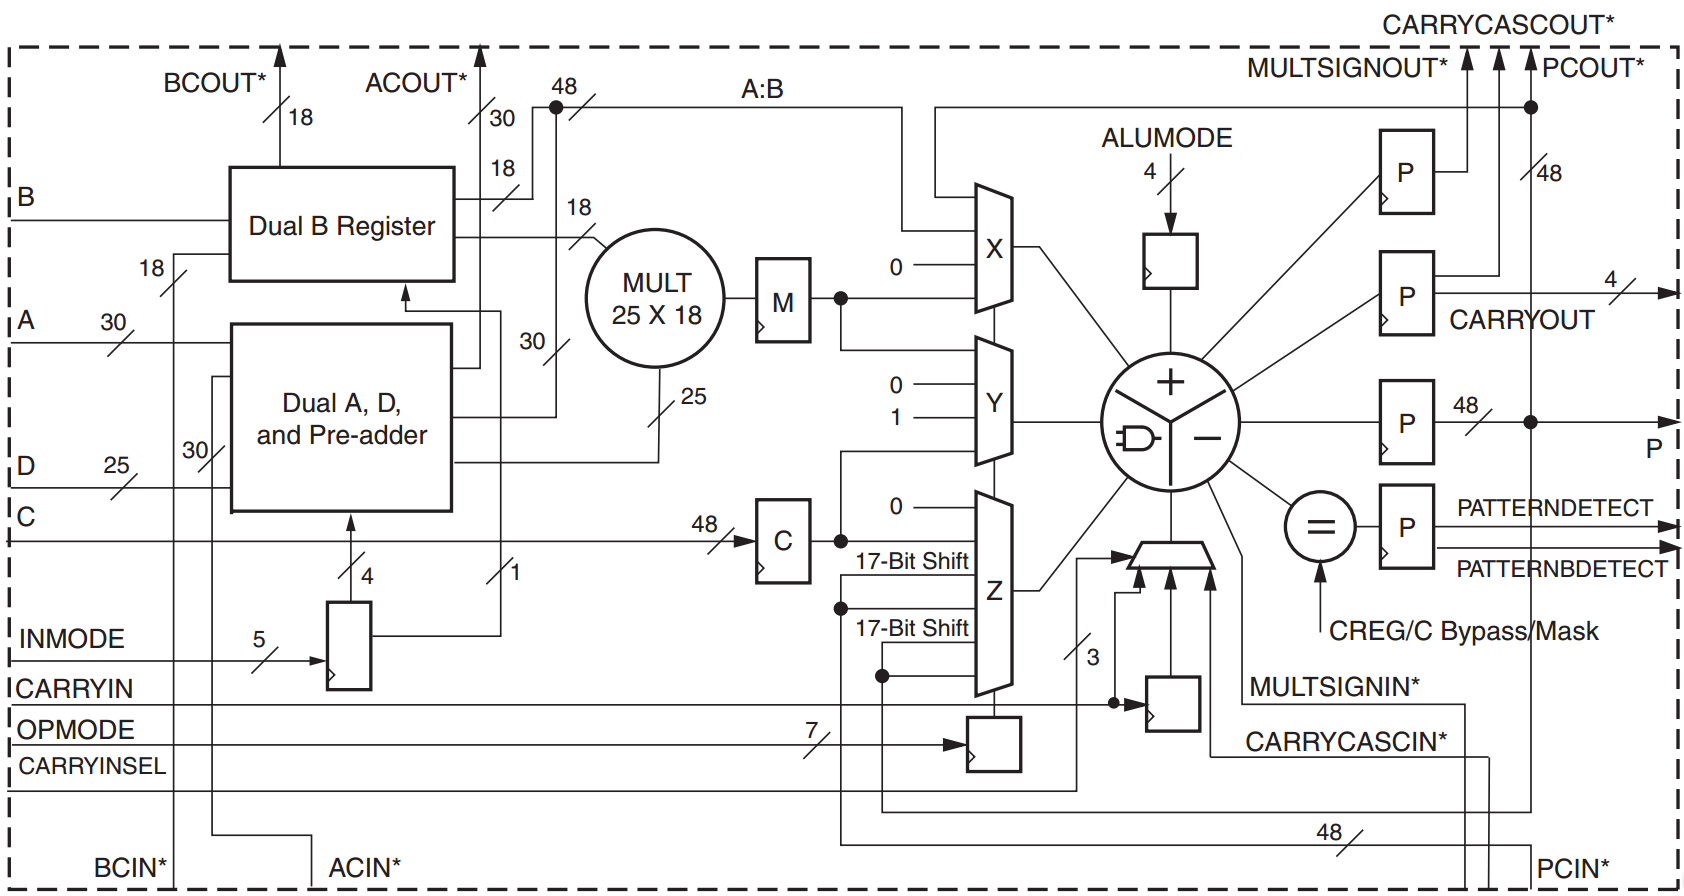
\includegraphics[width=\textwidth]{img/II-5-irradiation/dsp.png}
        \caption{Diagram of the DSP48E1 slices present in the Xilinx Virtex-6 family \cite{VIRTEX-DSP}.}
        \label{fig:II-5-dsp}
      \end{figure}

    \subsection{The Switching Matrix}

      The inputs and outputs of the slices of the CLBs as well as of the other components of the FPGA are interconnected through the switching matrix. It is a vast network of wires and switches which are used to route signals between elements. The open or closed state of each switch is programmable and defines the routes signals follow inside the logic. Figure \ref{fig:II-5-switch} shows an element of the matrix connected to two slices (blue) along with the signals that are routed in the network (cyan). Complex designs can span a large area of the FPGA due to the high usage of logic and thus be difficult to place and route by the compiler. A technique called floorplanning is used to reduce compilation time and improve the design by constraining parts of the code to given areas in the FPGA. This reduces propagation delays and logic usage which in turn yield a more efficient design.

      \begin{figure}[b!]
        \centering
        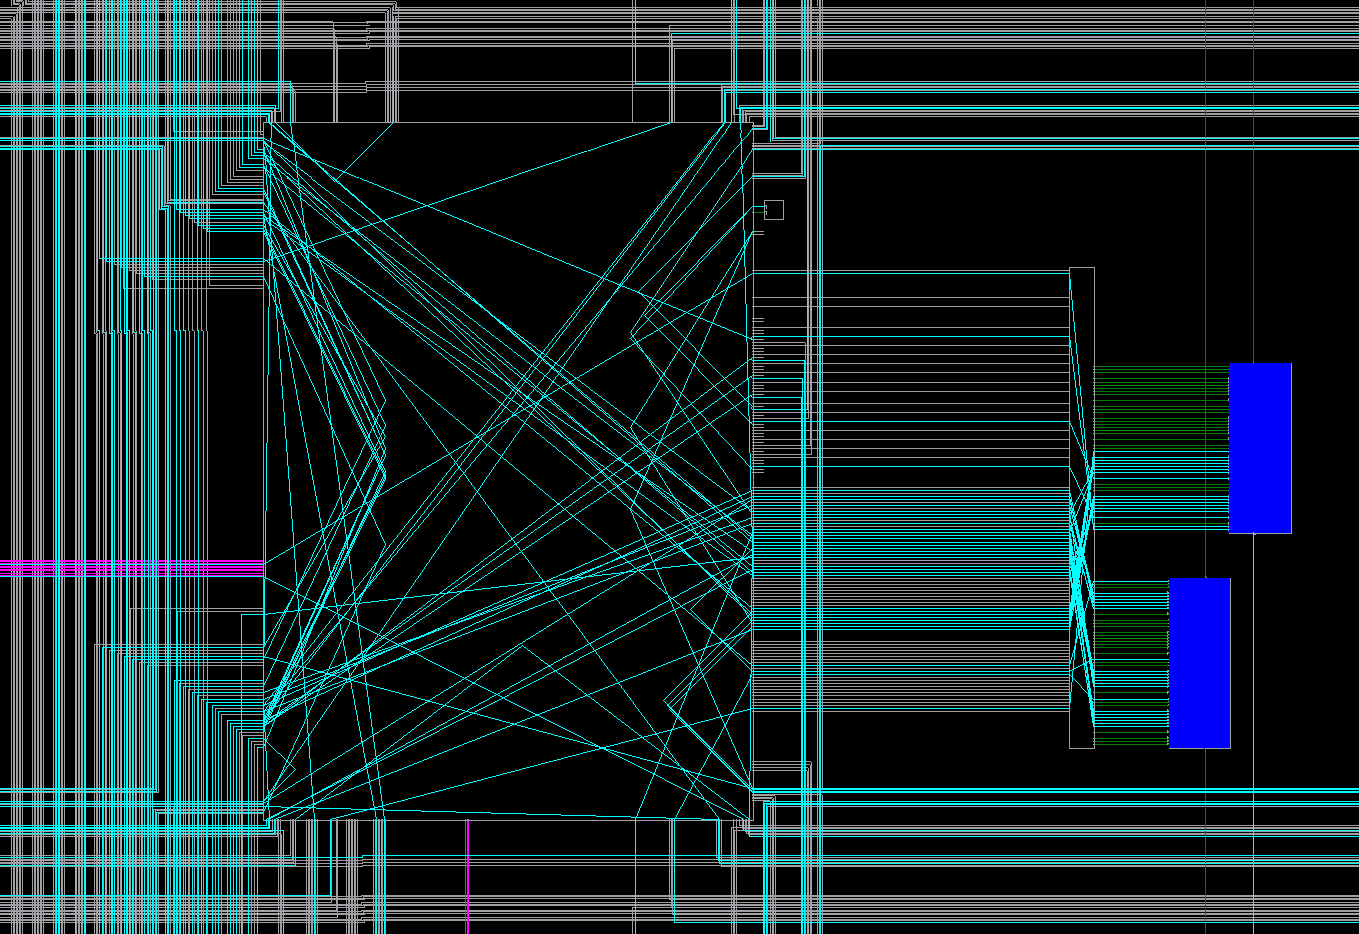
\includegraphics[width=\textwidth]{img/II-5-irradiation/switch.png}
        \caption{Schematic of two slices (blue) connected to an element of the switching matrix which routes the signals (cyan) between components over the multitude of existing paths (gray).}
        \label{fig:II-5-switch}
      \end{figure}

    \subsection{Block RAM (BRAM)}

      Besides programmable logic, the FPGA also includes dedicated storage elements. Block RAMs (BRAMs) \cite{VIRTEX-RAM} can store up to 36 kb of data which can be configured in different ways: 32K x 1 bit, 16K x 2 bits, etc. They can also be used as First In First Out (FIFO) modules which are similar to data queues.

    \subsection{The Configuration Memory}

      The configuration memory holds the configuration of the entire FPGA and defines its behavior. It sets the truth table of the LUTs, parametrizes the DSP, creates the connection between elements, etc. It is what implements the design in the FPGA. In most FPGAs, the configuration memory is volatile and will lose its content upon power down or reset. To reload it, the FPGA tries to read it out of an attached memory device or remains in a blank or corrupted state if it fails to do so.

  \section{Effects of Radiation on FPGAs}

    To understand how radiation affects an FPGA, it is import to know how the interaction between the particles and the silicon occurs and what the energy transfer mechanisms are. Then, the consequences of these energy depositions on the transistors of the chip can be analyzed along with the effects on the FPGA.

    \subsection{Energy Losses in Matter}

      Radiation affects the functioning of FPGAs through its interactions with the silicon substrate that composes the chip. These interactions take the form of direct or indirect ionization depending on the nature of the incident particle. Charged particles will directly ionize the medium through their Coulomb interactions with the electrons, causing them to escape with a fraction of the energy of the particle. Neutral hadrons on the other hand interact through indirect ionization which results from the scatterings with the medium which transfer energy to the electrons and nuclei. Both processes result in a trail of ions and electrons in the path of the incident particle. \\

      These energy losses are stochastic by nature and thus described by probability distributions around a mean value. They further depend upon the energy of the incident particle as different physical processes will have different behaviors for their cross sections. However, a value called the Linear Energy Transfer (LET) is used and defined as the amount of energy lost by a particle per unit of distance in the direct vicinity of the track
      \begin{equation}
        LET = - \frac{dE}{dX} .
      \end{equation}
      The latter greatly depends upon the medium and is thus normalized by its density and expressed in terms of MeV cm$^2$ g$^{-1}$. As reference, 62 MeV protons have a LET of 8.39 $\times$ 10$^{-3}$ MeV cm$^2$ mg$^{-1}$ while 33 MeV protons have a LET of 1.37 $\times$ 10$^{-2}$ MeV cm$^2$ mg$^{-1}$. The LET thus increases as the energy decreases due to the stronger interactions with the medium which will contain the energy deposition to a small cylinder around the track. The maximum LET is achieved when the particle comes to rest in the medium. High energy protons on the other hand will create $\delta$-rays inside the medium which will in turn create an ionization trail which does not contribute to the LET. The total deposited charge is thus higher and will have more impact on the devices.

    \subsection{Effects of Radiation on Transistors}

      The ions and electrons created along the track of the particle will either recombine if they are located in the bulk of the substrate, or drift towards the doped regions of the transistor if located near the p-n junction, as depicted in Figure \ref{fig:II-5-transistor}. The latter gives rise to the creation of an ion and electron current in the transistor and a resulting current spike at the gates of the component. This can propagate in the circuit and affect its status. \\

      \begin{figure}[b!]
        \centering
        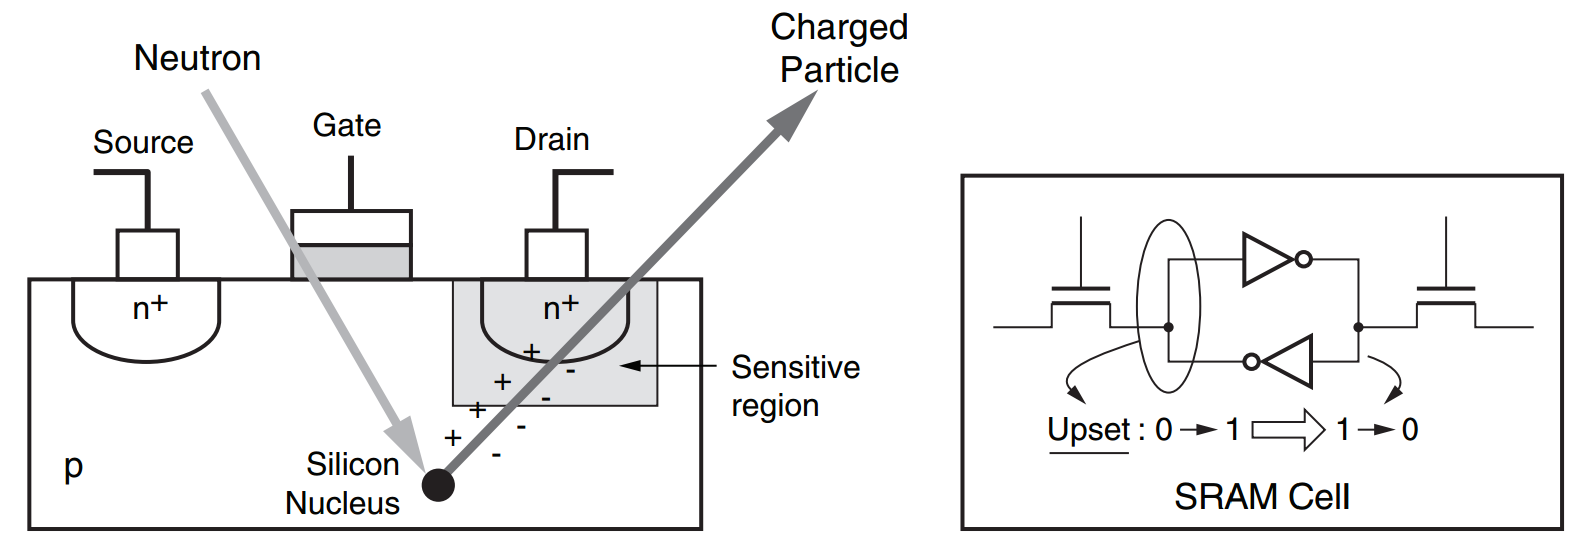
\includegraphics[width=0.5\textwidth]{img/II-5-irradiation/transistor.png}
        \caption{Charge deposition by a charged particle inside a transistor affecting the state of the circuit \cite{XILINX-RADIATION}.}
        \label{fig:II-5-transistor}
      \end{figure}

      Over time, charge builds up in the oxide region of the transistors and screens or enhances the electric field of the gate. This results in a shift of the voltage threshold of the transistor. Additionally, this also affects the mobility of the charge carriers in the region of the transistor where the conductive channel forms between the two doped regions. This can lead to current leakage and an increase in the voltage shift.

    \subsection{Single Event Transients (SET)}

      When a current spike occurs in a transistor due to the passage of a particle, it can be propagated inside the combinatorial logic of the device. These events are called Single Event Transients (SETs). They typically have a fast rising time on the order of 100 ps, and last for less than 1 ns. When coupled to sequential logic, such signals can easily be recovered from if their duration is small in comparison to the frequency of the clock used to run the circuit. Unless the error is produced exactly at the sampling time of the registers and thus sampled, it is not stored and thus mitigated. These errors are critical in purely combinatorial logic but can be easily mitigated in sequential logic. They will not be further discusses in the below sections.

    \subsection{Single Event Upsets (SEU)}

      If the transistor affected by the passage of a particle is located within a memory cell, the event is called a Single Event Upset (SEU). These events can trigger a change of state of the cell and result in a bit flip. Memory cells are composed of a group of transistors running in a stable state. They will retain their value until a change occurs or power is shut down. When an SEU occurs, the current spike causes the memory cell to react and place itself in another stable state, effectively operating a bit flip.

    \subsection{Total Ionizing Dose (TID)}

      With time, the amount of charge accumulated by the transistors increases and greatly reduces the efficiency of the device. The threshold voltage of the transistors is shifted such that they do not fulfill their function anymore and their behavior becomes unpredictable. This leads to a breakdown of the logic gates and thus the higher level functions they are part of. Sectors of the FPGA or the device itself might become unusable. These effects might dissipate over time if the device is removed from the irradiated area.

  \section{SEU Mitigation Techniques}

    To correct SEUs taking place in the configuration memory, the latter has to be read out by the FPGA itself. This is possible through the Soft Error Mitigation (SEM) core, a component placed inside the device which allows the firmware to analyze the data in memory and, using a two bit complement, perform a FEC on the bits. Although very effective to correct errors on the fly, this technique is time consuming due to the large amount of data to readout and can take up to several milliseconds to identify and repair an error. Furthermore, the FEC will fail to recover the data in case two bits are flipped within the same word, raising a flag that tells the system a hard reset is needed. While the error remains uncorrected, the components of the FPGA configured through the corrupted bits will encounter errors. \\

    A common technique used to mitigate errors in CLBs and DSPs is to triplicate the logic and couple its outputs to a majority voter. This allows to correct the data while SEM solves the corrupted bits in the configuration memory. First, the sequential logic is triplicated, meaning the inputs are sent to three identical modules which output is returned synchronously. The latter are then forwarded to a majority voter which performs a bit-by-bit vote and returns the most probable response. This technique can recover data if only one of the modules is affected by an SEU. In case two modules are corrupted and flip the same bit, data will be corrupted as well. Additionally, a flag can be raised by the majority voter if all three inputs are not identical, meaning an error occurred. A logic diagram of a triplicated module is shown in Figure \ref{fig:II-5-tmr}. Next to the simple triplication method exposed here-above and represented in black, a more complex triplication can be set in place and is represented in gray. In addition to the triplication of the modules holding the logic, the voter is also triplicated along with its outputs. In that scheme, the three outputs are passed to the next module on three different inputs. This allows to mitigate errors occurring in the voter itself. \\

    \begin{figure}[t!]
      \centering
      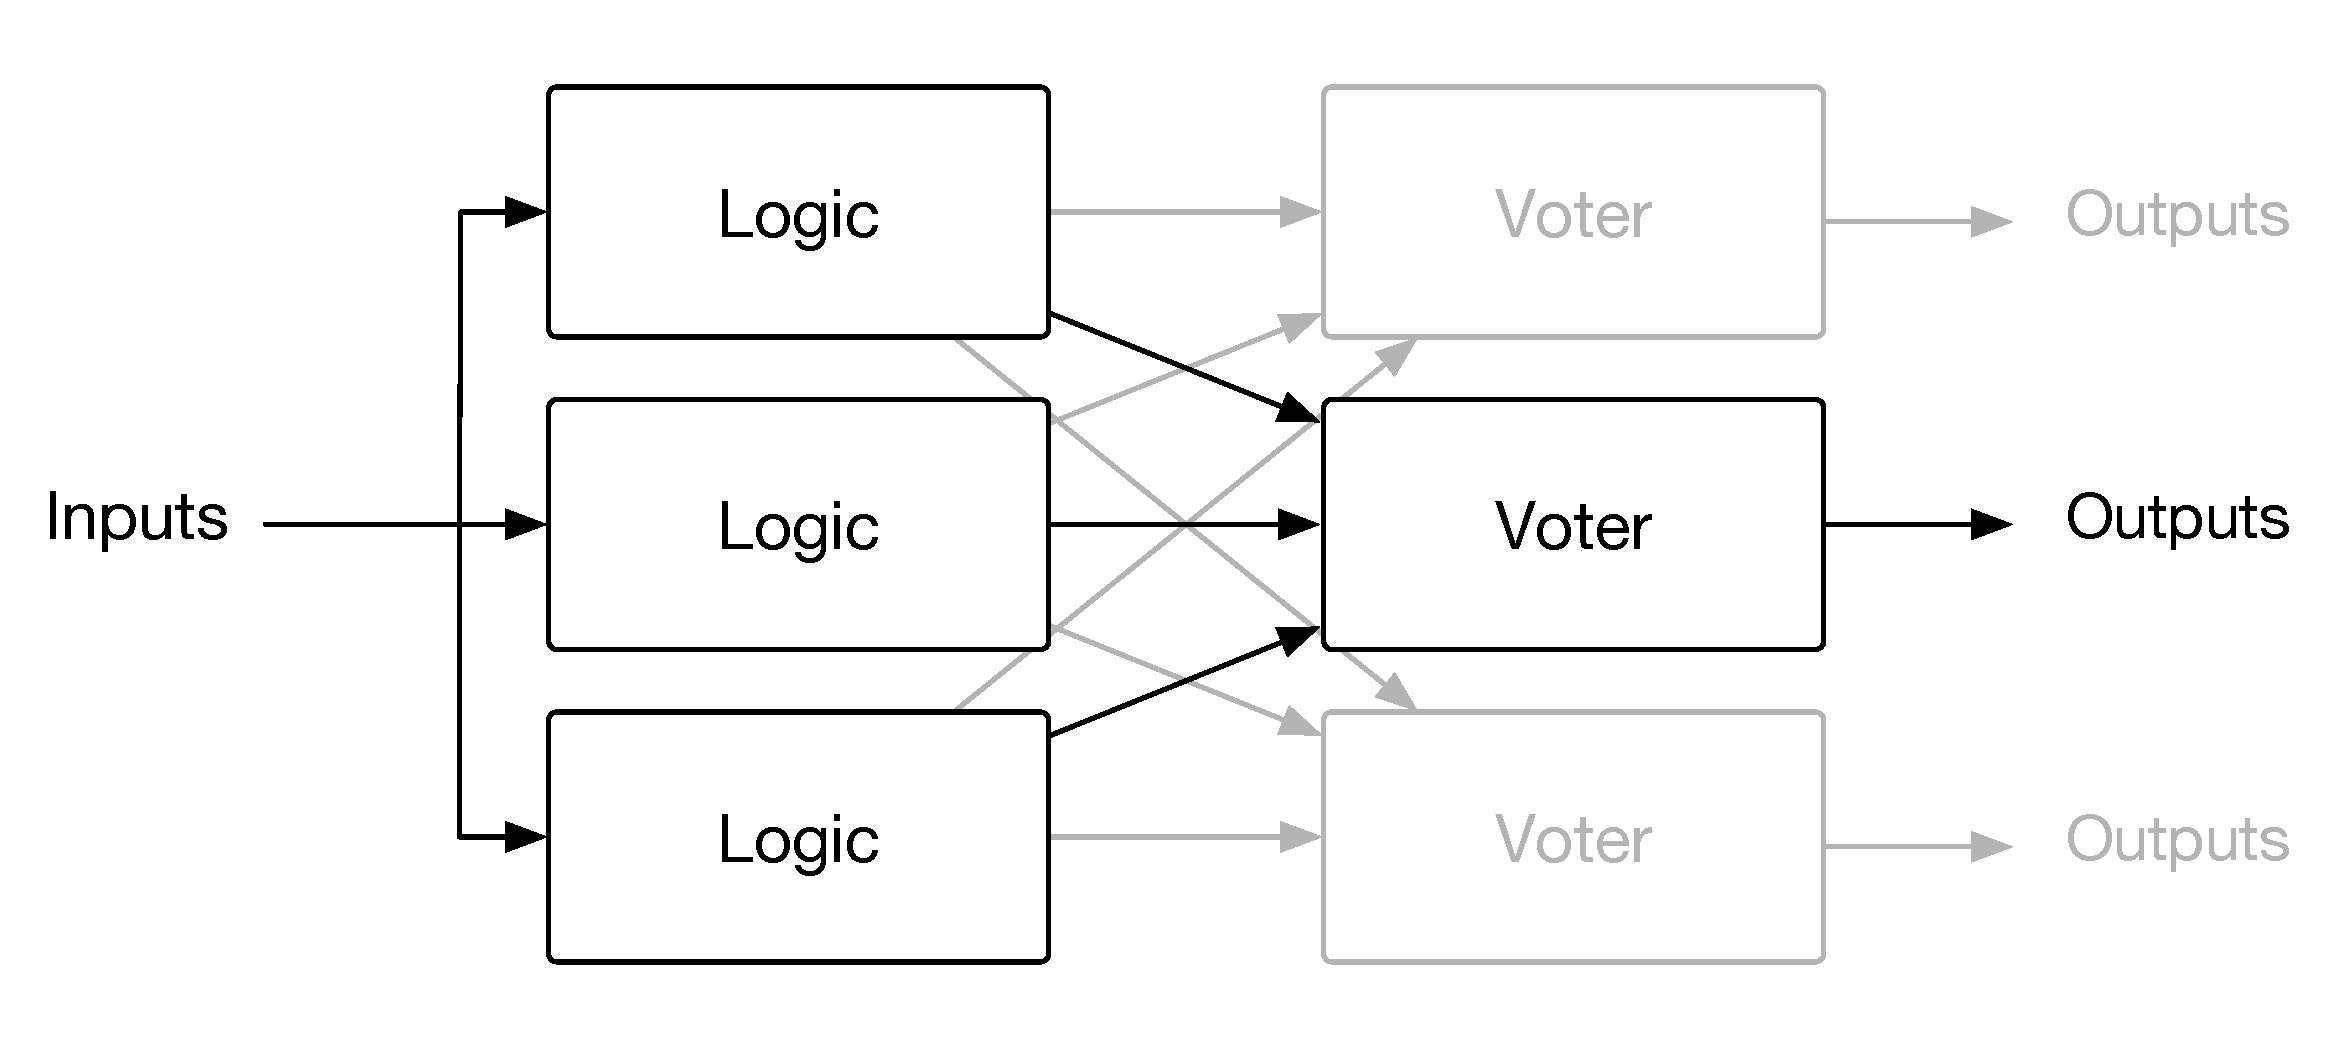
\includegraphics[width=0.7\textwidth]{img/II-5-irradiation/tmr}
      \caption{Logic diagram of a triplicated module coupled to a single voter (black) or to three distinct voters (gray).}
      \label{fig:II-5-tmr}
    \end{figure}

    Finally, SEUs occurring in BRAMs can be corrected using a two complements FEC which can recover single bit errors and detect double bit errors. This option is available on some BRAM components in the FPGA.

  \section{Firmware Design for the Irradiated FPGA}

    The firmware of the irradiated FPGA is designed to use a maximum of the available resources and transmit any error detected during run time. Specific firmware has been developed to test the CLBs, BRAMs, DSPs, and SEM. To optimize the design, floorplanning is used to divide the FPGA in ten regions running identical code. This prevents the compiler from placing elements in different sectors of the device and thus increase routing resources. Figure \ref{fig:II-5-floorplanning} depicts how the design occupies the FPGA: the image on the left represents the FPGA sectors labeled XaYb composed of CLBs in dark blue, BRAMs in red, and DSPs in green; the image in the middle highlights the resources used by the design; and the image on the right shows how the firmware developed for each function occupies the FPGA with CLBs in blue, BRAMs in yellow, DSPs in red, SEM in purple, and the communication protocol in green. The sampling rate of the various error detection tools is of 40 MHz. Figure \ref{fig:II-5-firmware} provides a logic diagram of the firmware designed to detect errors in the various components of the irradiated FPGA.

    \begin{sidewaysfigure}[p!]
      \centering
      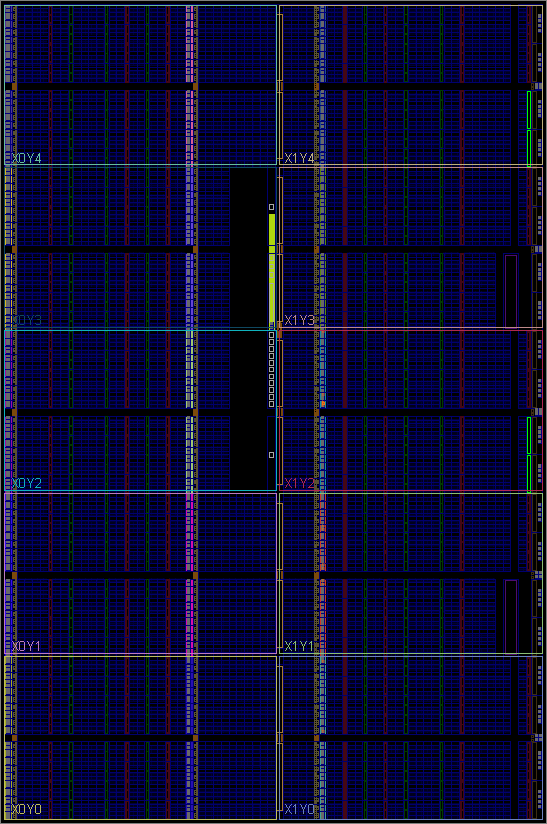
\includegraphics[width=0.32\textwidth]{img/II-5-irradiation/fpga-empty.png}
      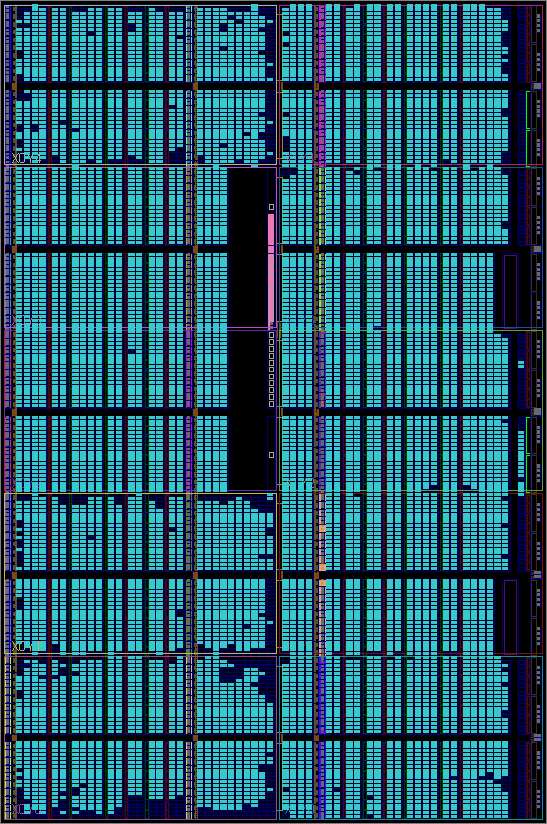
\includegraphics[width=0.32\textwidth]{img/II-5-irradiation/fpga-used.png}
      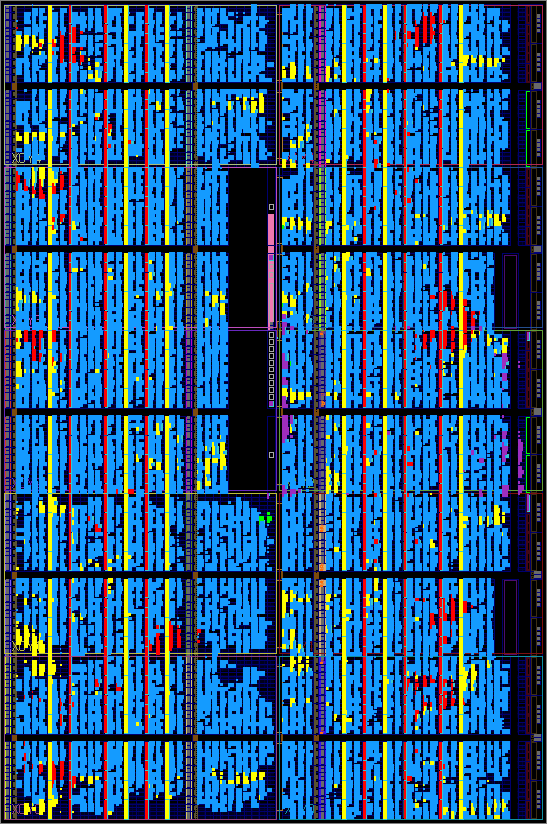
\includegraphics[width=0.32\textwidth]{img/II-5-irradiation/fpga-color.png}
      \caption{Schematic view of the occupancy of the FPGA. Left: sectors of the FPGA labeled XaYb composed of CLBs in dark blue, BRAMs in red, and DSPs in green. Middle: highlight of the resources used by the design. Right: occupancy of the code developed to test the CLBs in blue, BRAMs in yellow, DSPs in red, SEM in purple, and the communication protocol in green.}
      \label{fig:II-5-floorplanning}
    \end{sidewaysfigure}

    \begin{figure}[t!]
      \centering
      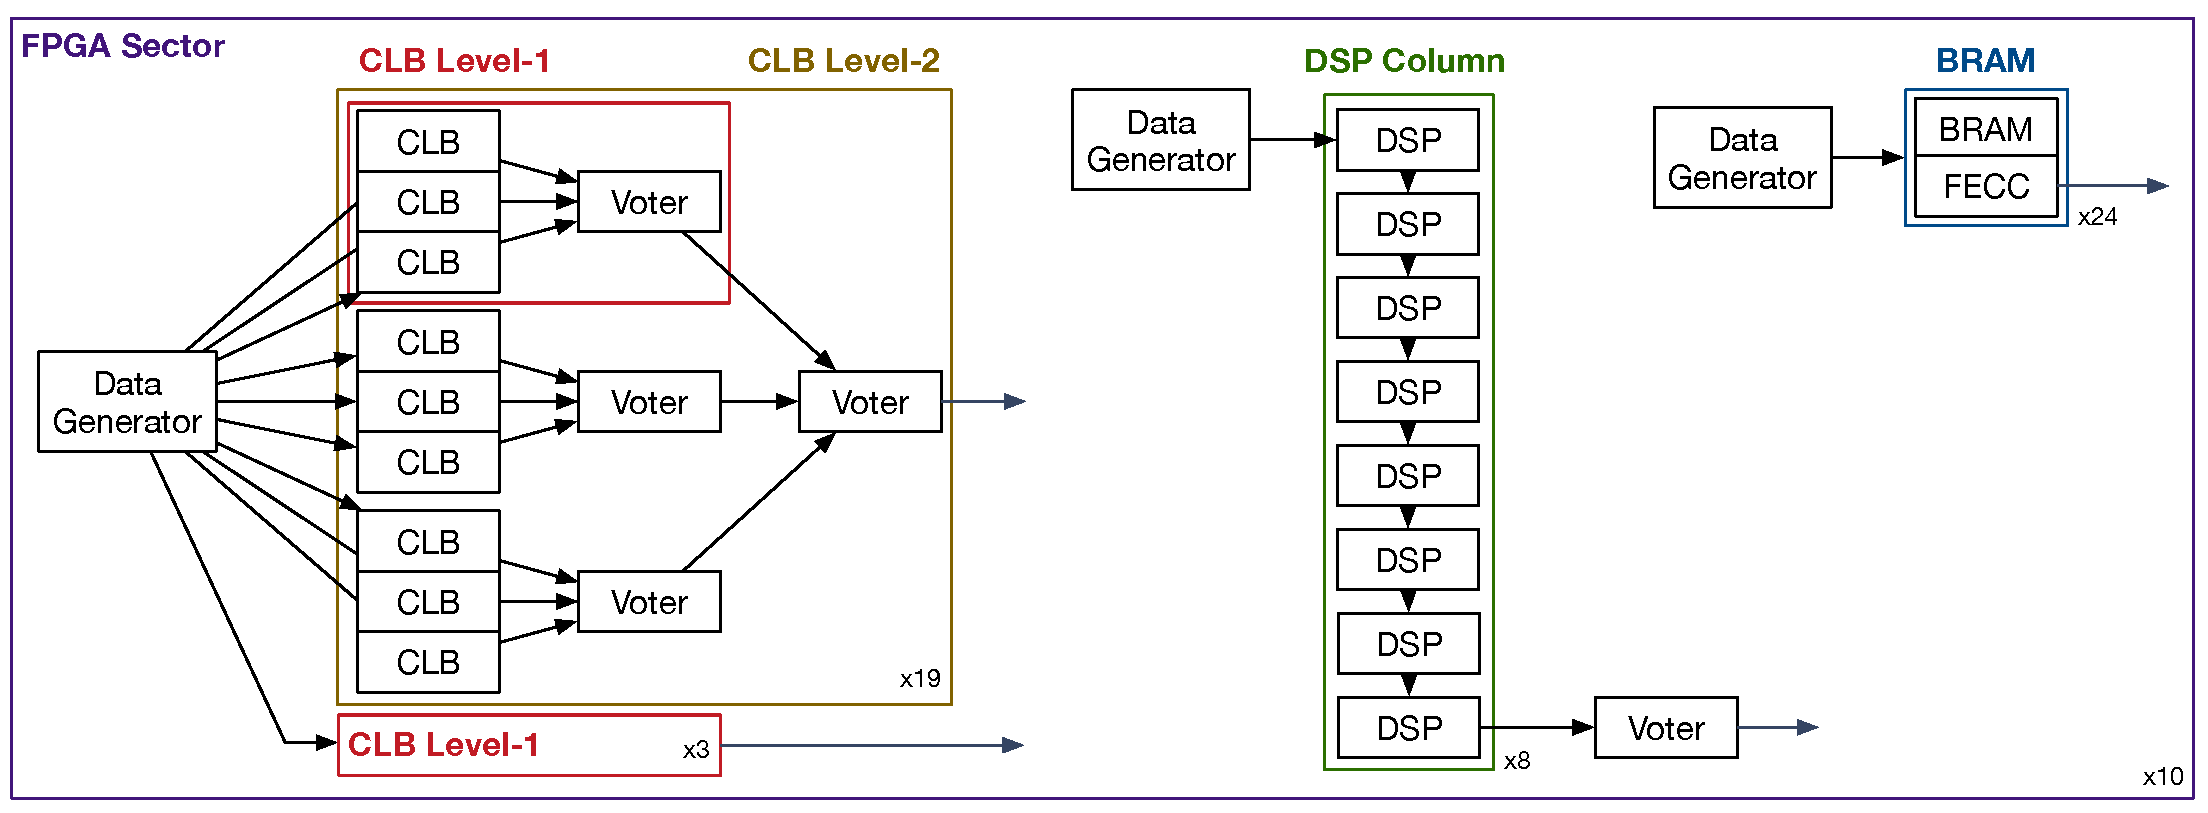
\includegraphics[width=\textwidth]{img/II-5-irradiation/firmware}
      \caption{Logic diagram of the firmware designed to detect errors in the irradiated FPGA.}
      \label{fig:II-5-firmware}
    \end{figure}

    \subsection{Configurable Logic Block}

      To test the CLBs, an algorithm performing logic operations and bit swapping on a 32-bit word is triplicated and connected to a majority voter to form a level-1 module. Three level-1 modules are connected together to another majority voter to form a level-2 module. The level-1 modules are used to detect errors in the CLBs and the level-2 modules to signal when the triplication technique fails to recover errors. The 32-bit word fed to the algorithm is generated by shifting a word every clock cycle. The same data is provided to all modules meaning that it is not susceptible to SEUs. \\

      Each of the 10 sectors of the FPGA contains 19 level-2 modules and 3 additional level-1 modules for a total occupancy of the FPGA of 80\%. Within each sector the flags of the level-1 and level-2 modules are gathered and sent to the communication module which forwards information to the control FPGA located outside the irradiation area of the tests.

    \subsection{Block RAM}

      In Xilinx Virtex-6 FPGAs, some of the BRAM components are equipped with error detection and correction features. These can detect double bit flips and correct for single bit flips. During the tests, 90\% of the available BRAMs, namely 240 components, are used and constantly written to and read from in order to detect SEUs happening inside the memory cells.

    \subsection{Digital Signal Processing}

      Each sector of the FPGA is composed of 48 DSPs grouped into 6 columns which share dedicated connections. Each column implements the same series of mathematical operations and is fed with the same 32-bit word generated within the sector. The results of the six columns are then compared to detect single, double, or triple failures according to the number of DSPs which returned a corrupted value.

    \subsection{Soft Error Mitigation}

      The SEM core included in the Xilinx Virtex-6 FPGA, when activated, continuously scans the configuration memory to detect corrupted bits. The core outputs various signals to report its status: a heartbeat, a detection flag which indicates an error has been identified, a correction flag which indicates an error has been corrected, and a critical flag which indicates the detected error cannot be recovered. In case the critical flag is set, a hard reset is needed to trigger a total reconfiguration of the FPGA from the external memory containing the design files.

  \section{Firmware Design for the Control FPGA}

    The signals collected by the irradiated FPGA are sent to a control FPGA located outside of the test area. This FPGA implements a set of counters that can be accessed by a computer through a dedicated core in the FPGA called ChipScope. The latter allows to monitor signals and send pulses inside the FPGA. It is used to monitor the communication protocol and read out the counters.

    \subsection{Communication Protocol}

      To connect the two boards, a High-Definition Multimedia Interface (HDMI) cable is used containing a total of eight wires. The data is always going from the irradiation zone to the control room with four of the wires used to send CLB, BRAM, and DSP errors and four used by the SEM core. \\

      The four wires used to transmit errors from the various components implement a simple protocol and encode data on two 4-bit words clocked at 40 MHz. The first word is composed of all '1' to inform the control FPGA that a communication is happening, and the second word encodes the type of error: CLB level-1, CLB level-2, BRAM single, BRAM double, DSP single, DSP double, or DSP triple. The control FPGA samples the signals at a frequency of 160 MHz in order to perform oversampling and avoid error when decoding the data due to the difference in frequency between the clocks of the two boards. \\

      The remaining four wires connected to the SEM core carry the heartbeat, detection, correction, and critical signals.

    \subsection{ChipScope Core}

      \begin{sidewaysfigure}[p!]
        \centering
        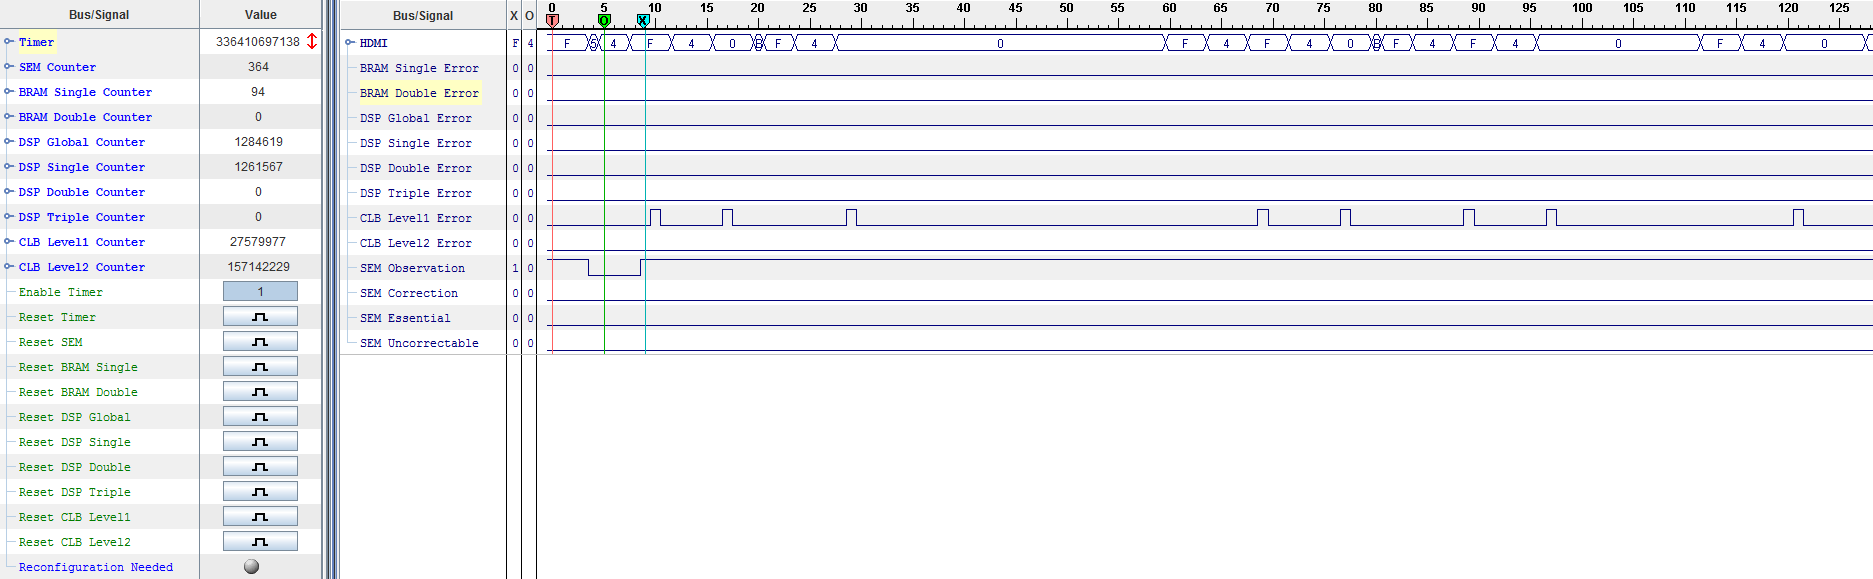
\includegraphics[width=\textwidth]{img/II-5-irradiation/cs-clb.png}
        \caption{View of the interface of ChipScope in which the VIO control window is located on the left where signals in blue are those that are read out, and signals in green are those that can be modified, and the ILA monitoring windows in shown on the right.}
        \label{fig:II-5-cs-clb}
      \end{sidewaysfigure}

      The Xilinx Virtex-6 FPGA implements a dedicated core called ChipScope that allows signals to be read out and set from a computer. In firmware, two versions of the core exist: one called Virtual Input/Output (VIO) which connects to signals and allows to modify or view them in real-time, and one called Integrated Logic Analyzer (ILA) which reads out the signals and provide a view of their evolution over time. In software, control windows can be created to handle those signals as depicted in Figure \ref{fig:II-5-cs-clb} in which the VIO control window is located on the left where signals in blue are those that are read out, and signals sin green are those that can be modified, and the ILA monitoring windows in showed on the right. \\

      The VIO window provides an overview of the error counters and allows to reset them individually. It also controls a timer which is used to count the elapsed time and a "reconfiguration needed" signal which indicates that the irradiated FPGA requires a hard reset. The ILA monitor displays the incoming bits and the resulting information. The first bus labeled "HDMI" holds the four bits used to encode the error types which can be seen to transition from 0x0 to 0xF and 0x4. The 0xF signals the beginning of a transmission and the 0x4 indicates a CLB level-1 error which in turn raises one of the error flags. The last four buses are connected to the signals of the SEM core.

  \section{Irradiation Setup}

    The irradiation tests were performed at the CYCLONE110 of the Cyclotron Resource Centre at the Université Catholique de Louvain \cite{CYCLOTRON} using a proton beam with energies between 14.4 MeV and 62 MeV. The machine can deliver fluxes up to 2 $ \times $ 10$^8$ particles cm$^{-2}$ s$^{-1}$ with a homogeneity of 10\% within an 80 mm of diameter beam spot. The top picture in Figure \ref{fig:II-5-cyclotron} is a photograph of the beam line delivering the protons in the irradiation area in front of which degraders can be placed in order to change the energy of the particles. The FPGA was the only component on the OptoHybrid to be directly exposed to the beam. \\

    \begin{figure}[p!]
      \centering
      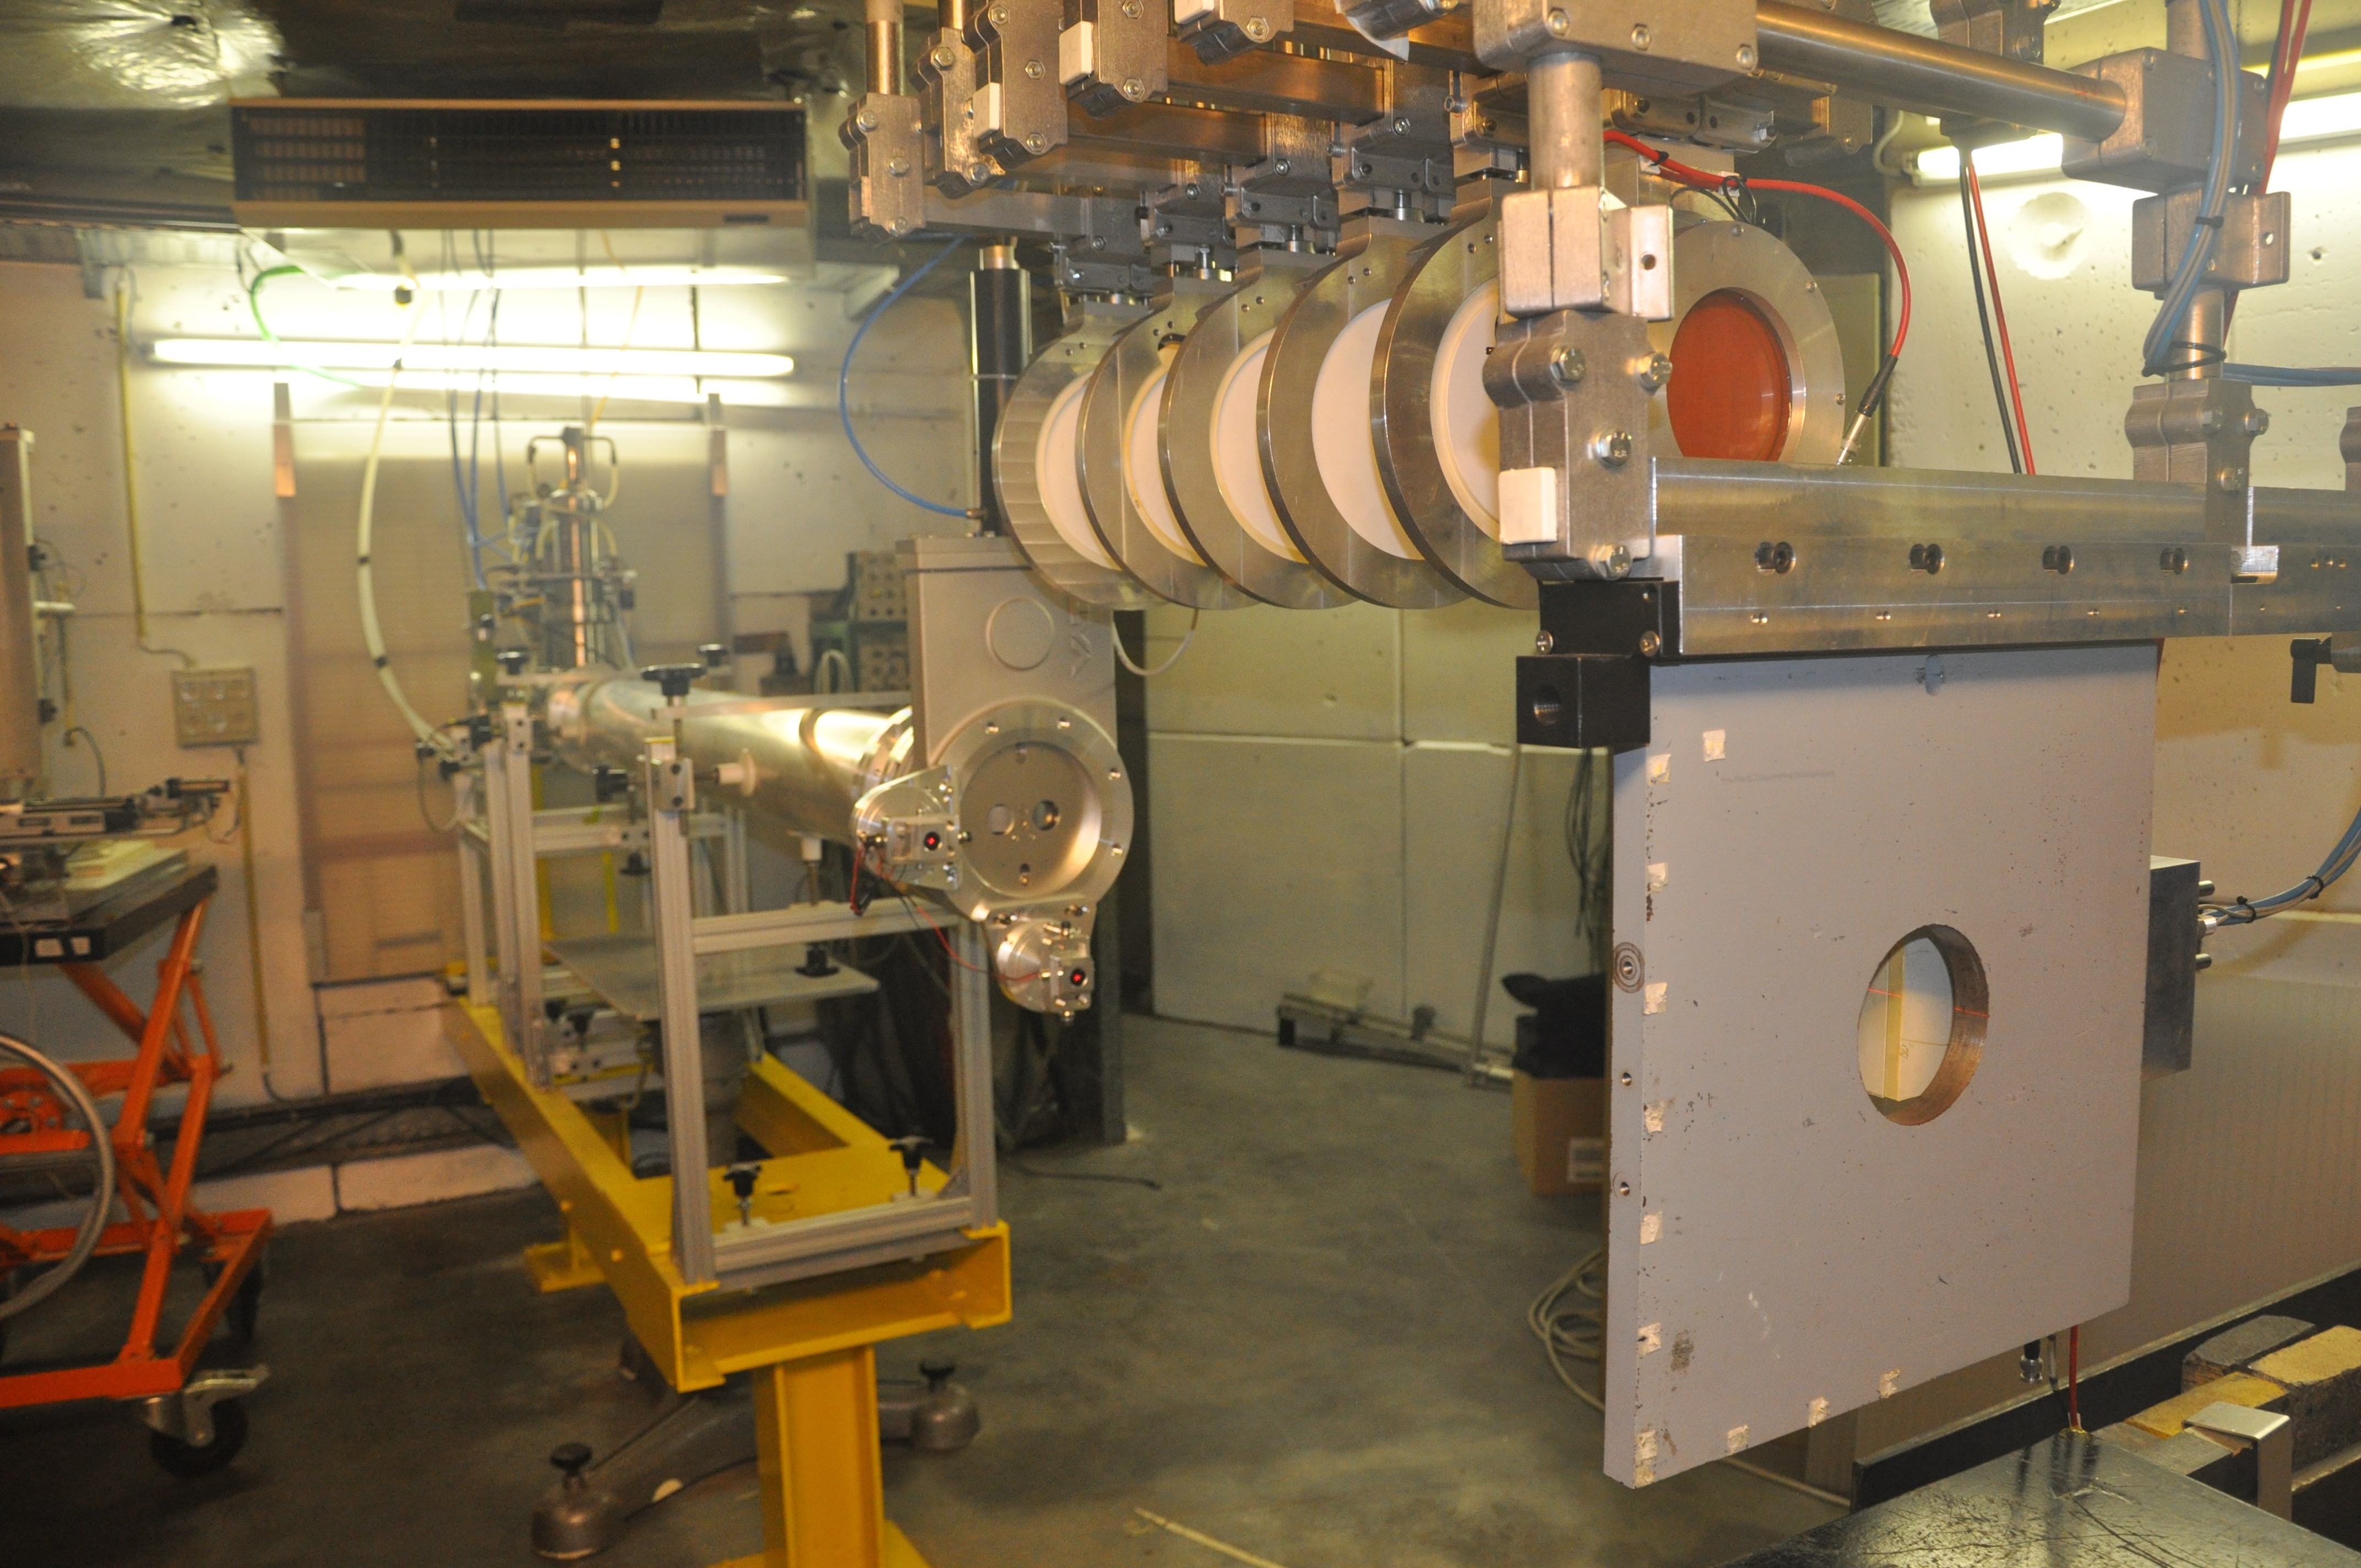
\includegraphics[width=\textwidth]{img/II-5-irradiation/cyclotron.jpg} \\
      \vspace*{0.4cm}
      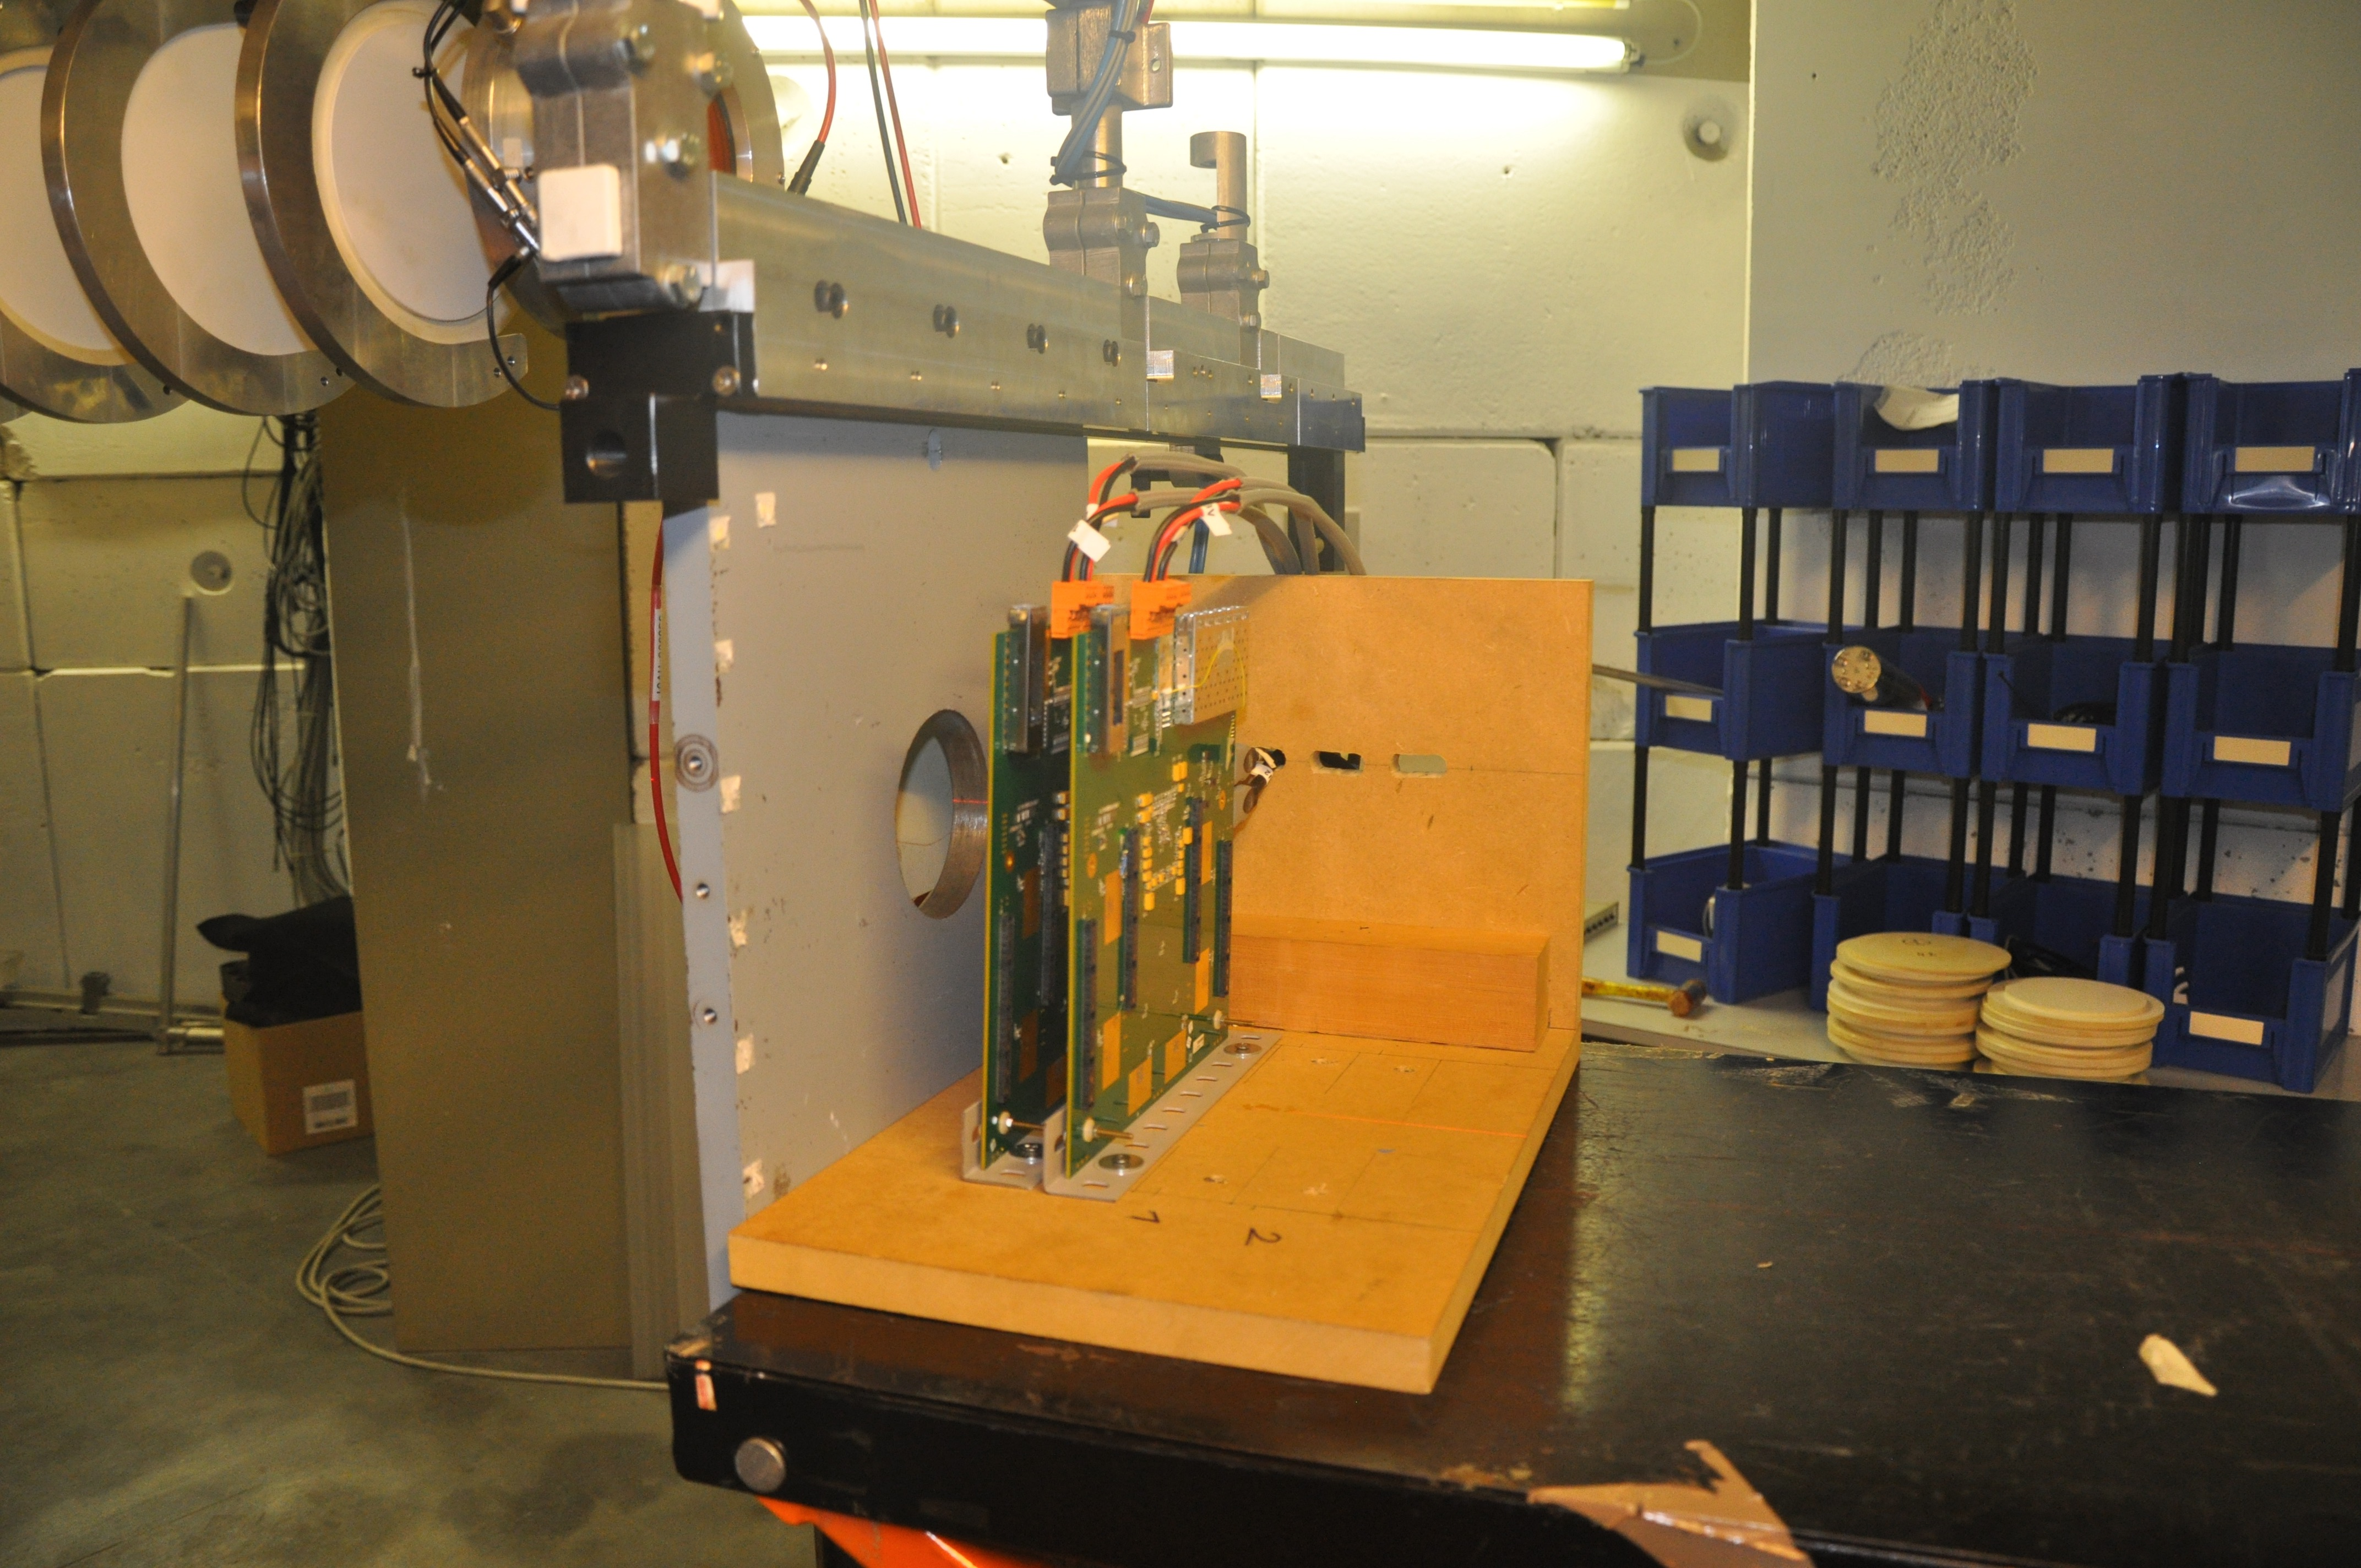
\includegraphics[width=\textwidth]{img/II-5-irradiation/boards.jpg}
      \caption{Top: photograph of the beam line delivering the protons in the irradiation area in front of which degraders can be placed in order to change the energy of the particles. Bottom: photograph of the two OptoHybrids being aligned in front of the beam using lasers.}
      \label{fig:II-5-cyclotron}
    \end{figure}

    Two OptoHybrids v2a were installed in front of the beam to mimic the setup of a superchamber in CMS. The bottom picture in Figure \ref{fig:II-5-cyclotron} is a photograph of the two boards being aligned in front of the beam using lasers. Next to the low voltage cables required to power the board, two HDMI cables are attached to each OptoHybrid v2a: one used to communicate with the control boards, and one used to send reset signals to the FPGA. \\

    In the control room, two additional OptoHybrids v2a were used to collect data through the HDMI cable and count the errors. These values were read out using ChipScope on the two control boards separately from a computer.

  \section{Data Analysis}

    The parameters of the beam and disposition of the setup allowed for the study of the dependence of the SEU cross section with the beam energy, TID, and placement of the boards. The number of SEUs was recorded for various energies and fluxes of particles over the course of 24 hours. For every case, the cross section was computed from the counters as being
    \begin{equation}
        \sigma = \frac{N}{\phi t} ,
    \end{equation}
    where $ N $ is the number of recorded SEUs, $ t $ is the duration of the test, and $ \phi $ is the flux of particles. \\

    Over the duration of the test, the TID of the FPGAs increased, reaching up to 84 krad. The rad is a unit used to measure the dose absorbed by the object and is a function of the fluence, which is the flux integrated over time, and of the LET. In comparison, the TID accumulated by the GE1/1 detectors in CMS at the end of Phase II is estimated to be of the order of 10 krad. To accelerate the aging process of the FPGAs and accumulate statistics, both boards were exposed to fluxes up to 10 000 times higher than those that they will have to cope within the environment of CMS. \\

    Finally, from the error counting in the CLBs and the two triplication levels, it is possible to extract the effectiveness of the latter method as mitigation technique of the SEUs.

    \subsection{Evolution of the SEU Cross Section with the Energy}

      The cross section with the configuration memory and the BRAMs were computed from the data collected using the results of the SEM core and the FEC of the BRAMs. Figure \ref{fig:II-5-data-seu-energy} displays the interaction cross section of particles as a function of the energy of the beam for the configuration memory resulting in recoverable (green) and critical (blue) errors on the left, and with the BRAMs resulting in single (blue) and double (orange) bit flips on the right. \\

      \begin{figure}[b!]
        \centering
        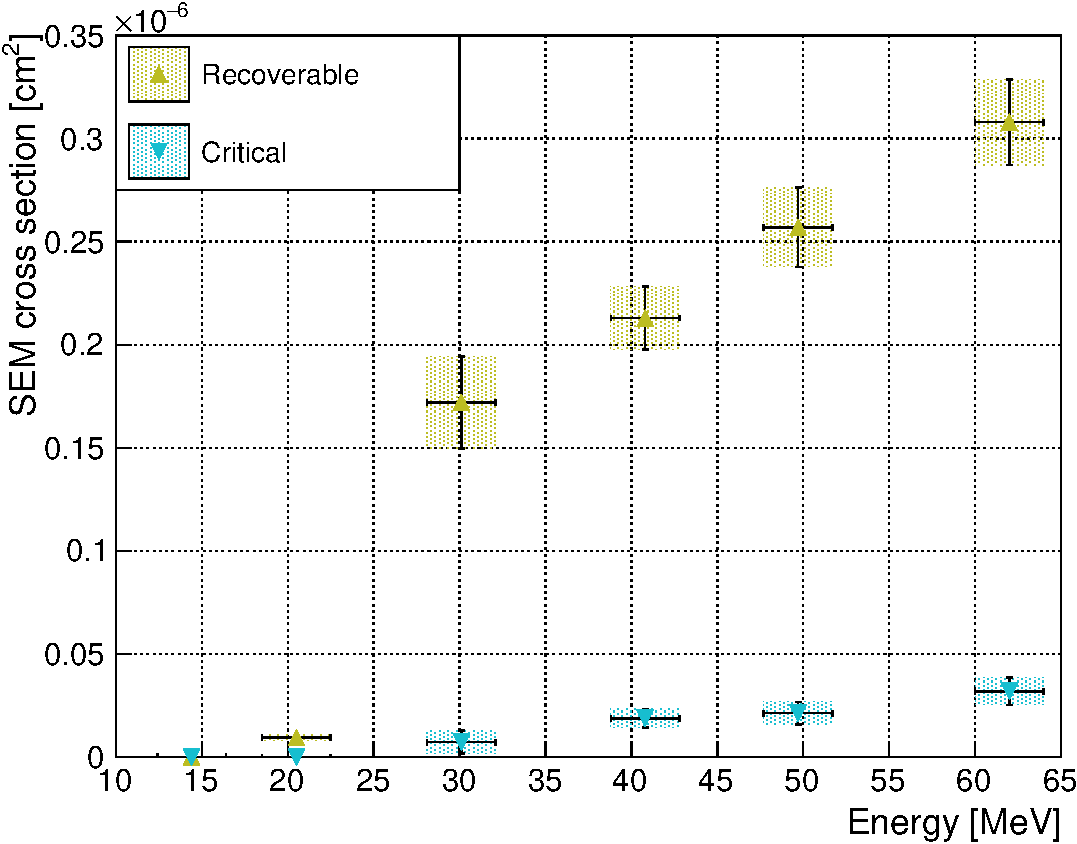
\includegraphics[width=0.49\textwidth]{img/plots/cE_SEM-crop}
        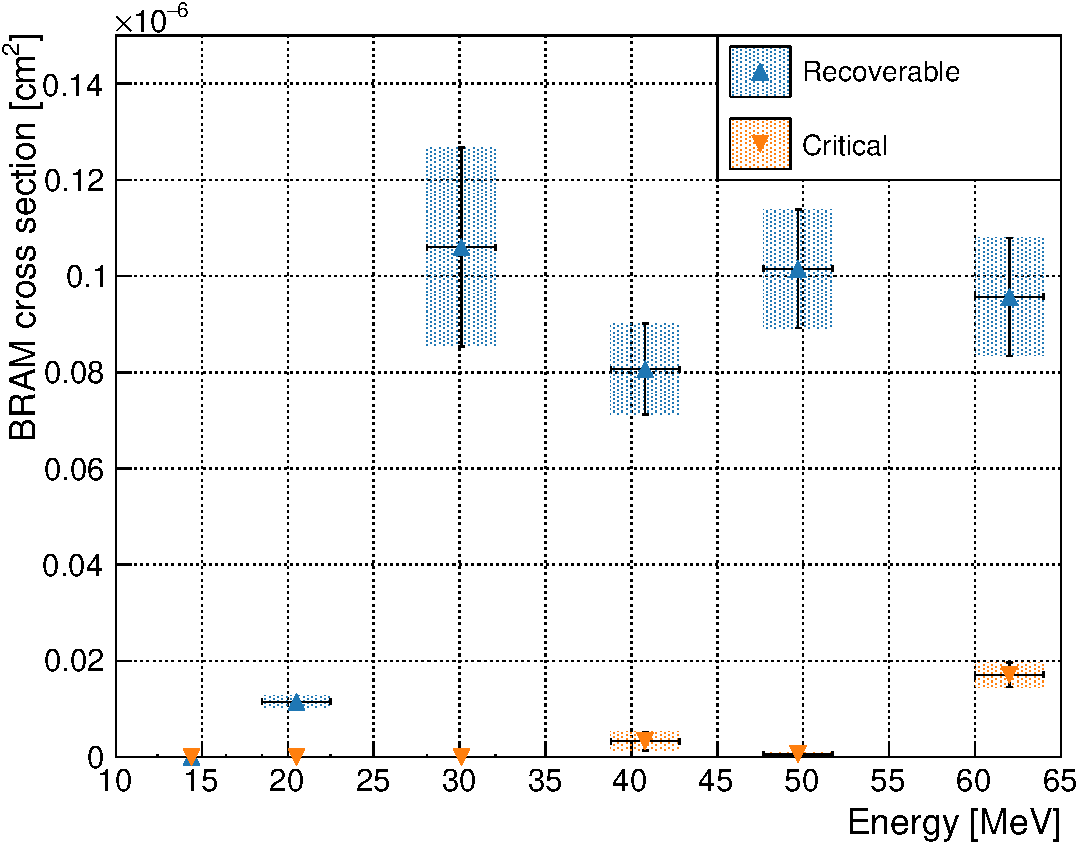
\includegraphics[width=0.49\textwidth]{img/plots/cE_BRAM-crop}
        \caption{Interaction cross section of particles as a function of the energy of the beam for the configuration memory resulting in recoverable (green) and critical (blue) errors on the left, and with the BRAMs resulting in recoverable (blue) and critical (orange) errors on the right.}
        \label{fig:II-5-data-seu-energy}
      \end{figure}

      Under 20 MeV, the number of errors is almost null with a cross section less than 1.14 $\times$ 10$^{-8}$ cm$^2$, in both the configuration memory and BRAMs, with zero errors detected at the lowest energy of 14.4 MeV. This behavior has been observed and explained in previous irradiation tests \cite{Bylsma2013242, Huhtinen2000155} and is due to the very limited range of the particles. At 10 MeV, protons have a LET of 3.48 $\times$ 10$^{-2}$ MeV cm$^2$ mg$^{-1}$, and can only penetrate the first 10 $\mu$m in silicon due to the high energy losses they experience. They are thus not able to interact with the core of the FPGA but only with its packaging. At higher energies, the particles start to penetrate the silicon and recoverable errors are detected while critical errors are still rare events with a cross section of 1.88 $ \times $ 10$^{-8}$ cm$^2$ for protons of 40.8 MeV in the configuration memory. The latter are still rare as the total deposited energy is low and only reaches a limited range in the fabric of the FPGA. This generate single bit flips which result in recoverable errors. At even higher energies, above 40 MeV, the number of SEUs in the configuration memory keeps increasing to reach a cross section of 3.08 $\pm$ 0.21 $ \times $ 10$^{-7}$ cm$^2$ at 62 MeV while the error count in the BRAM seems to hit a plateau at a cross section of 1.02 $\pm$ 0.12 $ \times $ 10$^{-7}$ cm$^2$. \\

      These results can be compared with tests performed for the electronics of the CSCs \cite{Bylsma2013242} for the same FPGA, which yielded values of 3.7 $\pm$ 0.50 $ \times $ 10$^{-8}$ cm$^2$ and 5.7 $\pm$ 0.60 $ \times $ 10$^{-8}$ cm$^2$ for interaction cross sections with the CLBs and BRAMs respectively at 55 MeV. The discrepancy in the values obtained for the configuration memory and CLBs is expected as the measured quantities differ. The configuration memory encapsulates the CLB and other resources present in the FPGA. It is thus expected that the interaction cross section of the former be larger than the latter. Exact numbers relative to the percentage of memory that is used to describe the CLBs are not disclosed by Xilinx, only an estimate of 6.4\% is given \cite{XILINX-SEM}. This scaling factor can be applied to the cross section of the configuration memory at 62 MeV to find an approximative cross section for the CLBs of 1.98 ($\pm$ 0.14) $\times$ 10$^{-8}$ cm$^2$. For both the CLBs and the BRAMs, the obtained cross sections do not match within the error bars but however are at the same order of magnitude, only varying by a maximum of 50\%. \\

      Finally, a comparison with the reference values provided by Xilinx \cite{XILINX-RELAIBILITY} can be done. The latter uses the irradiation facility of the Los Alamos Neutron Science Center to produce a neutron beam with an energy spectrum similar to the one measured in the atmosphere. The resulting neutrons range in energy from 0.1 MeV to 1 GeV with an unknown flux. A strict comparison cannot be performed, however, a validity check on the order of magnitude of the results is possible. The reference document states a cross section of 1.26 $\pm$ 0.23 $\times$ 10$^{-14}$ cm$^2$ per bit of configuration memory. The FPGA used in the design of the OptoHybrid holds 43 720 728 bits resulting in a cross section for the entire FPGA of 5.51 $\pm$ 0.99 $\times$ 10$^{-7}$ cm$^2$. This is compatible with the value obtained of 3.08 $\pm$ 0.21 $ \times $ 10$^{-7}$ cm$^2$ at energy of 62 MeV. The same can be done for the BRAM, for which a cross section of 1.14 $\pm$ 0.21 $ \times $ 10$^{-14}$ cm$^2$ per bit of memory is announced. This yields a cross section of 9.84 $\pm$ 0.18 $\times$ 10$^{-8}$ cm$^2$ for the entire FPGA. This can be put in parallel with the value of 1.02 $\pm$ 0.12 $ \times $ 10$^{-7}$ cm$^2$ obtained in this study. The values for the configuration memory differ by less than 32\% while the values of the BRAM are within the error margins. This validates the experimental process and results presented here-above.

    \subsection{Evolution of the SEU Cross Section with the TID}

      The OptoHybrids were initially exposed to a total of 33 krad over the course of various tests performed during the first 22h. The remaining two hours were used to irradiate the FPGAs with high fluxes and then perform a data taking run to measure a potential increase in interaction cross section: first, three runs that each provided 10 krad, followed by a run at 20 krad. Figure \ref{fig:II-5-data-seu-tid} displays the interaction cross section of particles as a function of the TID at an energy of 49.7 MeV for the configuration memory resulting in recoverable (green) and critical (blue) errors on the left, and with the BRAMs resulting in recoverable (blue) and critical (orange) errors on the right. \\

      \begin{figure}[t!]
        \centering
        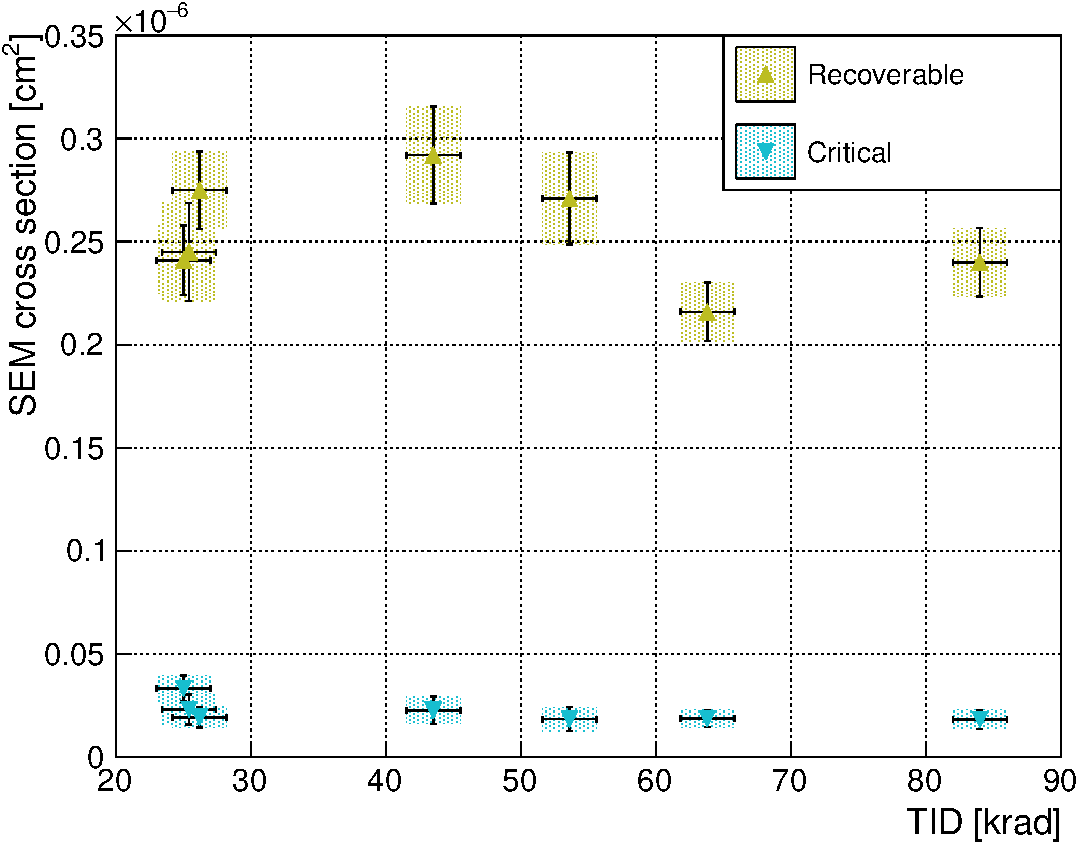
\includegraphics[width=0.49\textwidth]{img/plots/cDose_SEM-crop}
        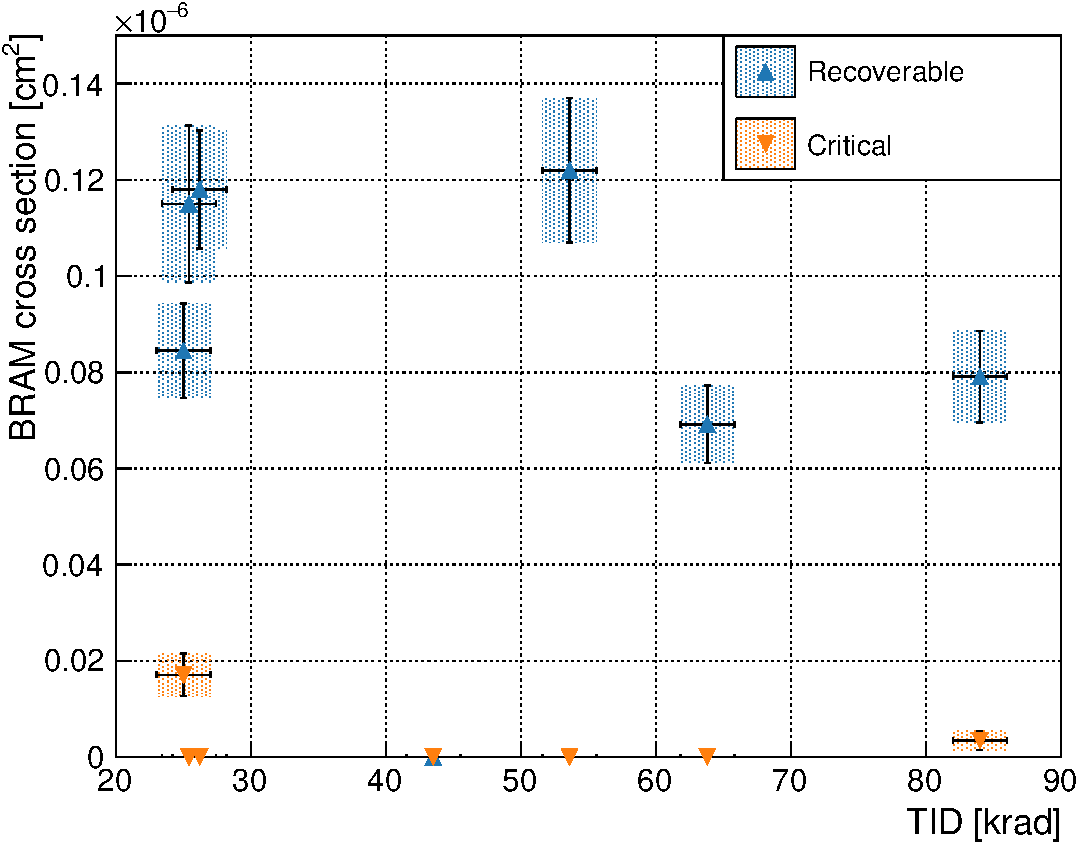
\includegraphics[width=0.49\textwidth]{img/plots/cDose_BRAM-crop}
        \caption{Interaction cross section of particles as a function of the TID at an energy of 49.7 MeV for the configuration memory resulting in recoverable (green) and critical (blue) errors on the left, and with the BRAMs resulting in recoverable (blue) and critical (orange) errors on the right.}
        \label{fig:II-5-data-seu-tid}
      \end{figure}

      From these results, no trend indicating an increase of the interaction cross section with the TID has been observed. This means that the FPGA remains operational at radiation doses that exceed those expected at CMS. Similar conclusions have been made from previous irradiation tests \cite{Bylsma2013242} were the TID reached 30 krad.

    \subsection{Evolution of the SEU Cross Section with the In-Beam Position}

      A comparison between the two boards was operated regarding the evolution of the interaction cross section with the energy. A different behavior is expected from the two FPGAs as the first one shields the second one at low energies. As particles pass through the former, they lose energy and might reach the threshold at which no SEU is produced in the latter. Figure \ref{fig:II-5-data-seu-comp} displays the interaction cross section of particles as a function of the energy of the beam and the position of the FPGA for the configuration memory resulting in recoverable (green and red) and critical (blue and purple) errors on the left, and with the BRAMs resulting in recoverable (blue and green) and critical (orange and red) errors on the right. \\

      \begin{figure}[t!]
        \centering
        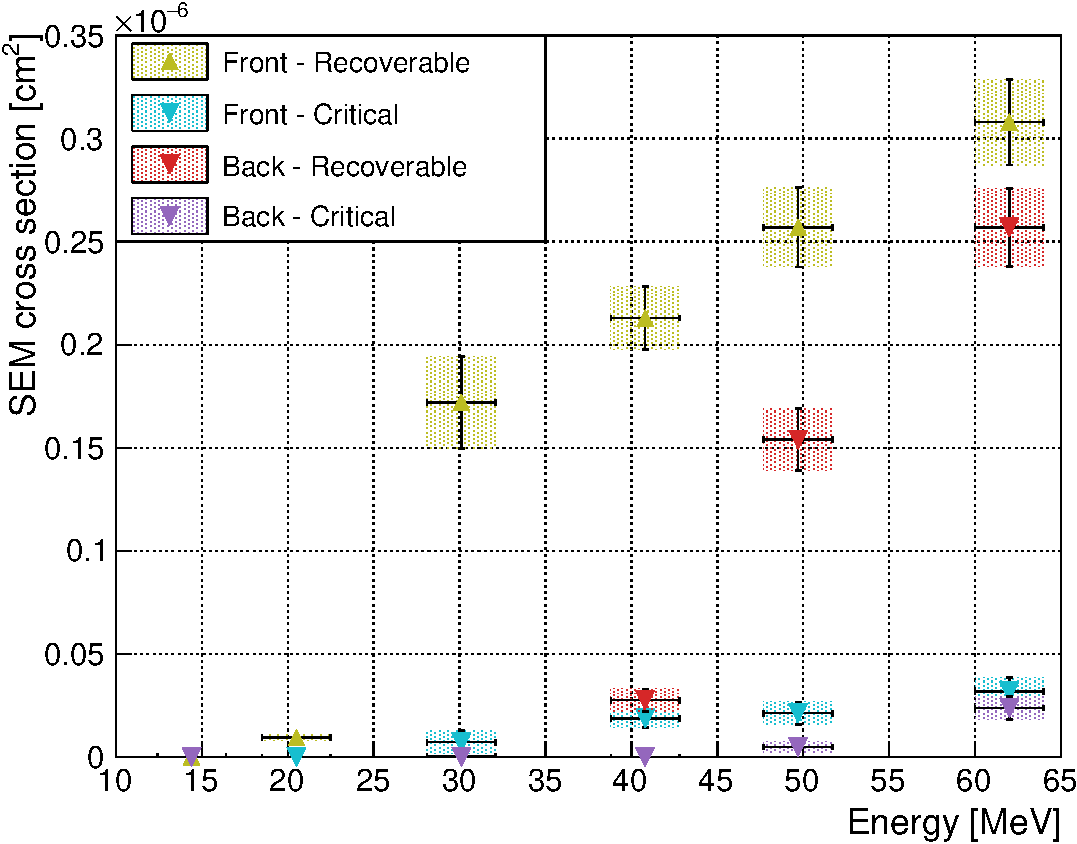
\includegraphics[width=0.49\textwidth]{img/plots/cE_SEU_Comp-crop}
        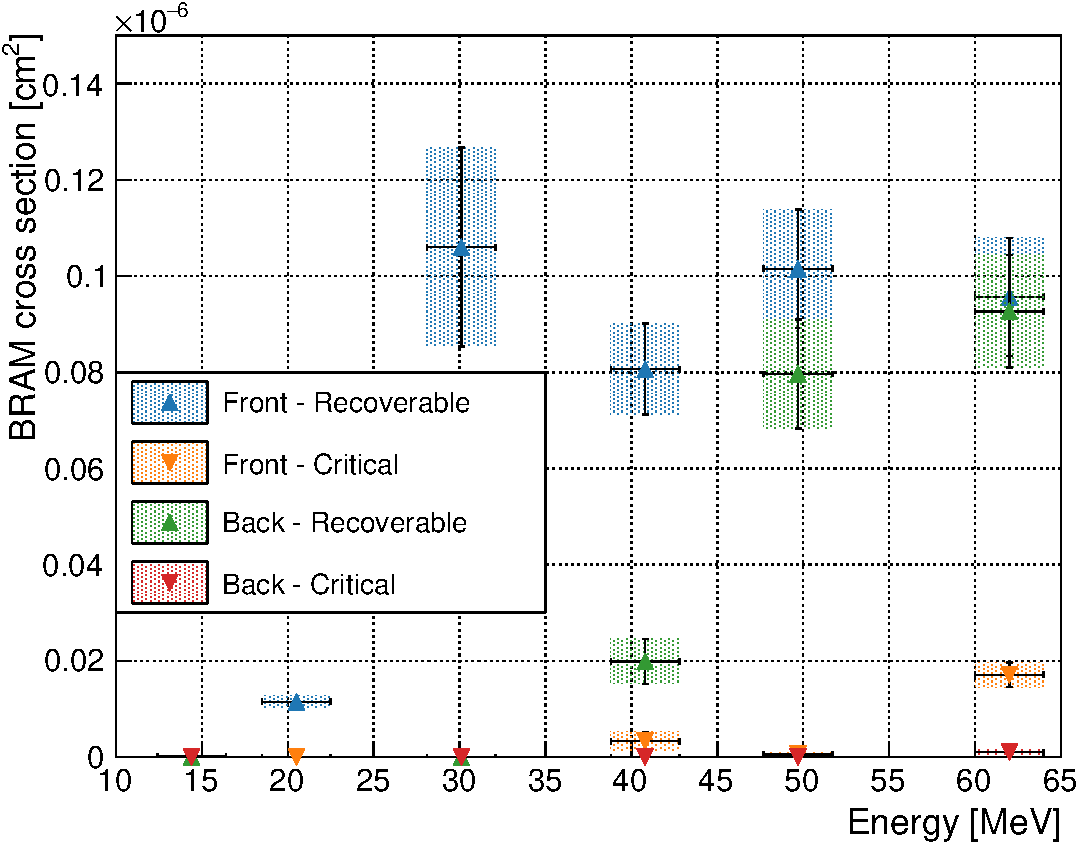
\includegraphics[width=0.49\textwidth]{img/plots/cE_BRAM_Comp-crop}
        \caption{Interaction cross section of particles as a function of the energy of the beam and the position of the FPGA for the configuration memory resulting in recoverable (green and red) and critical (blue and purple) errors on the left, and with the BRAMs resulting in recoverable (blue and green) and critical (orange and red) errors on the right.}
        \label{fig:II-5-data-seu-comp}
      \end{figure}

      It can be seen that the interaction cross section with the configuration memory of the second FPGA is lower than the first one due to the shielding provided by the latter. An incident beam with less than 40 MeV will not impact the second OptoHybrid due to the low energy remaining in the beam after the first interaction. The effect becomes visible only at energies higher than 40 MeV where the slope of the curve quickly rises. The interaction cross section with the BRAM displayed a plateau in the first FPGA, which is also seen in the second one, with the only difference being in the energy at which it appears. \\

      To confirm the fact that no errors are expected in the second FPGA at energies below 40 MeV, the energy losses of the particles through the first FPGA can be computed using the LET. At 40 MeV, the LET is of 1.17 $ \times $ 10$^{-2} $ MeV cm$^2$ g$^{-1}$. From the specifications of the Xilinx Virtex-6 FPGAs, it can be found that the chip is made of a 1-mm-thick silicon layer, with density of 2.3290 g cm$^{-3}$, protected by a 1-mm-thick copper lid, with a density of 8.96 g cm$^{-3}$. The PCB of the OptoHybrid adds an additional 1.8 mm of FR-4 material with a density of 1.850 g cm$^{-3}$. Using these number, a total energy loss can be computed
      \begin{equation}
        \Delta E = LET \times \rho \times h,
      \end{equation}
      where $\rho$ is the density of the material and $ h $ its thickness. The combined energy loss is of 17.71 MeV for a particle of 40 MeV. This means it will have an energy of 22.29 MeV when reaching the second FPGA and thus be at the energy threshold to produce an SEU.

    \subsection{Interaction with the CLBs and DSPs}

      The errors occurring in the CLBs and DSPs are due to bit flips in the configuration memory which change the structure of the design. This means that these SEUs will be detected by both SEM and the triplicated logic. By computing the ratio of errors seen in the CLBs and DSPs, and by making the approximation that all errors produced in the configuration memory are reflected in either of these components, an upper limit can be given on the interaction cross section. From all the events recorded by the triplicated logic, 6.61\% affected the DSPs and 93.39\% the CLBs. By applying those ratios to the cross section of recoverable errors in SEM, this yields an interaction cross section of 2.04 $ \times $ 10$^{-8}$ cm$^2$ and 2.88 $ \times $ 10$^{-7}$ cm$^2$ respectively for protons at 62 MeV.

    \subsection{Effectiveness of Triplication as Error Mitigation Technique}

      The effectiveness of this method was tested during irradiation at various particle fluxes. For this, two levels of triplication were compared: the level-1 which triplicates a basic algorithm, and the level-2 which triplicates the level-1 modules resulting in a double level of triplication. A failure of the level-1 only indicates that an error was detected in one of the module but corrected by the method. A failure detected at the level-2 is a sign that the triplication failed to correct an error in the system. Using these signals, a failure and success rate can be computed for this technique. Figure \ref{fig:II-5-data-triplication} shows the success (blue) and failure (orange) percentage of the triplication method according to the flux of particles when an SEU appears. \\

      \begin{figure}[h!]
        \centering
        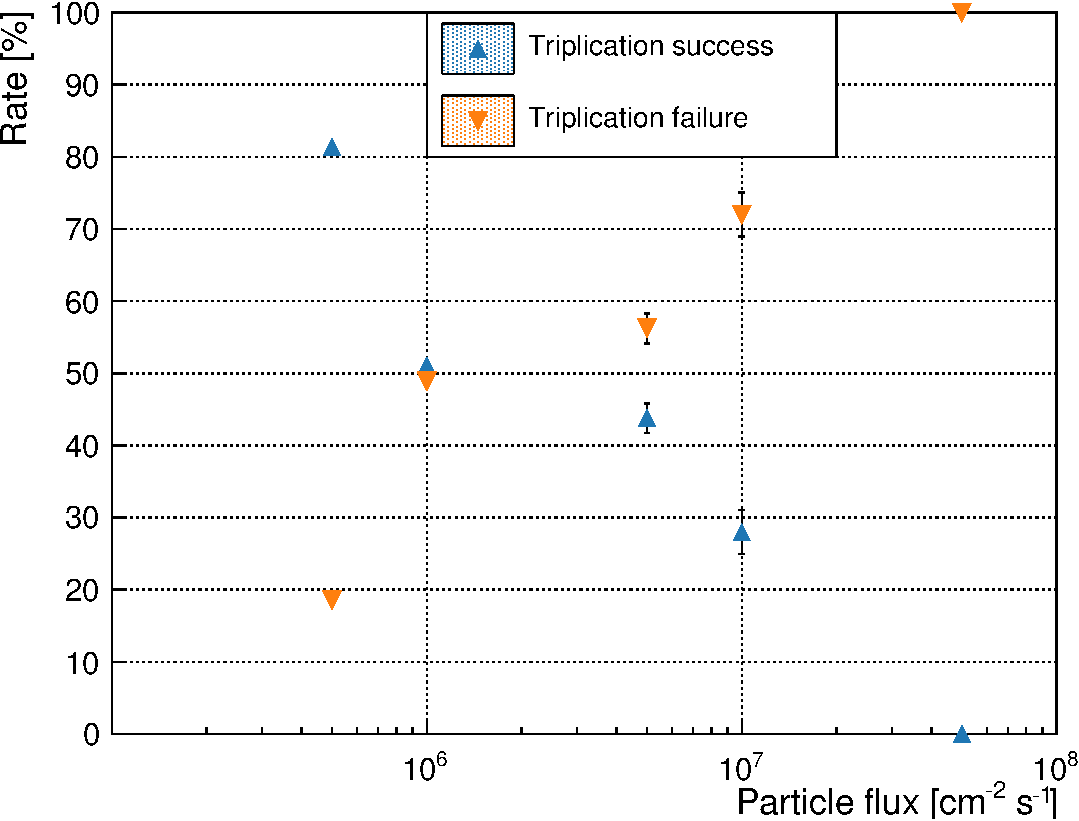
\includegraphics[width=0.49\textwidth]{img/plots/c_l-crop}
        \caption{Success (blue) and failure (orange) percentage of the triplication method according to the flux of particles when an SEU appears.}
        \label{fig:II-5-data-triplication}
      \end{figure}

      As can be observed, the failure rate increases with the particle flux due to the accumulation of errors in the design. The characteristic time needed to correct an error in the configuration memory is of a few milliseconds which at high fluxes is longer than the time between two SEUs. If two SEUs affect the same area of the logic, the triplication method will fail. At fluxes of 5 $ \times $ 10$^7$ cm$^{-2}$ s$^{-1}$, the SEU rate is so high that the triplication method cannot recover data at all. However, by extrapolating the data points, it can be seen that this technique will prove efficient and mitigate the SEUs at fluxes below 10$^5$ cm$^{-2}$ s$^{-1}$.

    \subsection{Impact on the Triple-GEM Upgrade Project}

      From the numbers obtained during the irradiation tests, it is possible to estimate the number of SEUs that will be observed by the OptoHybrid in GE1/1 during run time in CMS. The dominant background in CMS is composed of photons and neutrons. Figure \ref{fig:II-5-neutrons} shows the particle fluxes for the GE1/1 station as a function of the pseudorapidity for the LHC Phase II on the left, and the energy spectrum of the background particles in GE1/1 on the right. \\

      \begin{figure}[t!]
        \centering
        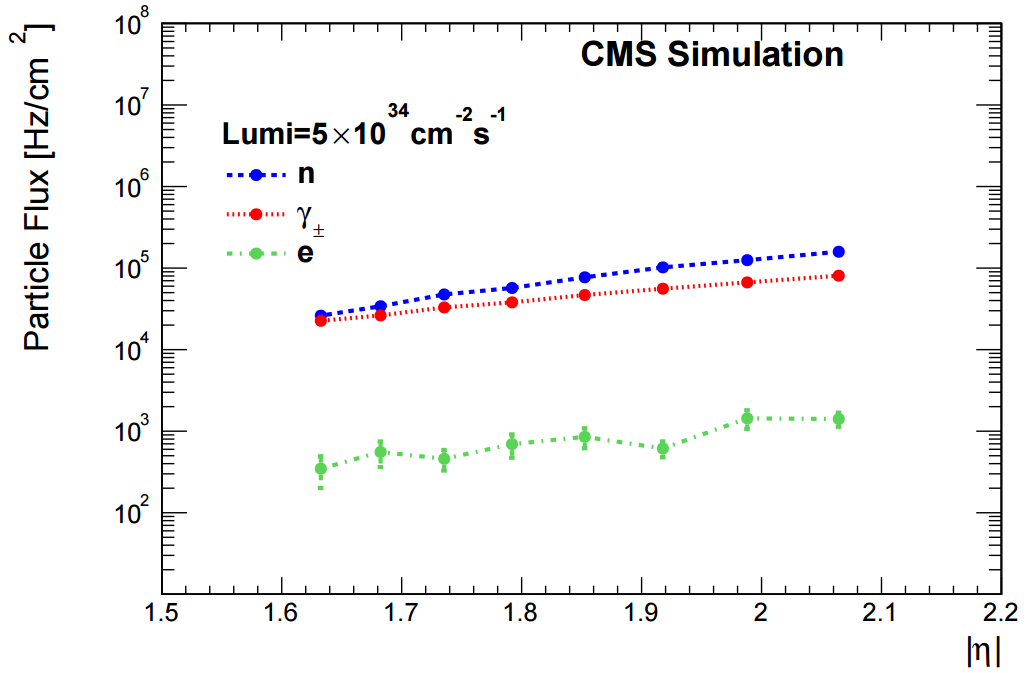
\includegraphics[width=\textwidth]{img/II-5-irradiation/fluka.png}
        \caption{Left: particle fluxes for the GE1/1 station as a function of the pseudorapidity for the LHC Phase II \cite{Zenoni:2065693}.Right: energy spectrum of the background particles in GE1/1 \cite{Zenoni:2065693}.}
        \label{fig:II-5-neutrons}
      \end{figure}

      The fluxes shown on the left are integrated over the whole energy spectrum and reach a maximum around 100 kHz cm$^{-2}$ for photons and neutrons at the highest $\eta$ value of 2.1. The OptoHybrid will be located in the lowest $\eta$ region where fluxes reach 20 kHz cm$^{-2}$. These values have to be corrected according to the energy of the incident particles and the type of interactions they undergo with the FPGA. Photons do not interact with the silicon of the FPGA as the thickness of the chip (< 1 mm) is four orders of magnitude smaller than their mean free path in silicon (12 cm) \cite{Agashe:2014kda}. Experimental results \cite{trad} showed that electrons have an interaction cross section with silicon devices five orders of magnitudes lower than protons. These results coupled with the flux of electrons which is around 200 Hz cm$^{-2}$ leads to a negligible contribution of the electrons with less than one event per year. Finally, neutrons can be described with the same values as those obtained for protons as they lead to similar rates of SEUs \cite{Huhtinen2000155}. \\

       The 20 kHz cm$^{-2}$ flux is thus reduced as the contribution from the particles below 20 MeV is ignored as it has been shown that they do not interact with the FPGA. Therefore, in order to set an upper limit on the number of SEUs, the interaction cross section is integrated with the flux between 20 MeV and 1 GeV. The cross section for particles with energy higher than 62 MeV is linearly extrapolated from the results shown in Figure \ref{fig:II-5-data-seu-energy}. Table \ref{tab:II-5-seu-rate} lists the types of SEUs encountered along with their respective interaction cross section and the resulting rate of errors in CMS per FPGA for the LHC Phase I ($ \mathcal{L} $ = 2 $\times$ 10$^{34}$ cm$^{-2}$ s$^{-1}$) and LHC Phase II ($ \mathcal{L} $ = 5 $ \times $ 10$^{34}$ cm$^{-2}$ s$^{-1}$) conditions. The LHC Phase II conditions correspond to a fluxes 2.5 times higher than for LHC Phase I. \\

      \begin{table}[h!]
        \begin{tabularx}{\textwidth}{L{1.1}C{1}C{0.95}C{0.95}}
          \textbf{Event type} & \textbf{cross section} & \textbf{SEUs per day \newline LHC Phase I} & \textbf{SEUs per day \newline LHC Phase II} \\ \hline
          SEM - recoverable & 3.08 $ \times $ 10$^{-7}$ cm$^2$ &  13.3  & 33.2  \\
          SEM - critical & 3.19 $ \times $ 10$^{-8}$ cm$^2$ & 1.36  & 3.44  \\
          BRAM - recoverable & 1.02 $ \times $ 10$^{-7}$ cm$^2$ & 4.38  & 11  \\
          BRAM - critical & 1.71 $ \times $ 10$^{-8}$ cm$^2$ & 0.54  & 1.33  \\
          CLB & 2.88 $ \times $ 10$^{-7}$ cm$^2$ & 12.42  & 31  \\
          DSP & 2.04 $ \times $ 10$^{-8}$ cm$^2$ & 0.88  & 2.2 \\
        \end{tabularx}
        \caption{Types of SEUs encountered along with their respective interaction cross section and the resulting daily rate of errors in CMS per FPGA assuming that the LHC runs at nominal values during 24h.}
        \label{tab:II-5-seu-rate}
      \end{table}

      The recoverable errors do not pose a problem for the design as the triplication method can be used to successfully mitigate all errors in the CLBs and DSPs caused by the configuration memory, and ECC can correct those in the BRAM. Indeed, the maximum flux of 2 kHz cm$^{-2}$ is inferior to the 100 kHz cm$^{-2}$ the triplication can handle. The critical errors will require a partial reconfiguration of the FPGA, a process in which the defective bits are recovered from the external memory device and reloaded in real-time. Finally, the double bit flips in the BRAM can be mitigated by triplicating the storage of data in memory, which is allowed due to the large amount of available BRAMs.

    \subsection{Impact on the Firmware of the OptoHybrid}

      The presented results are upper limits on the cross section of SEUs for an FPGA which resources are fully used. The firmware of the OptoHybrid v2 used for the DAQ system of the slice test occupies 36\% of the CLBs and 3\% of the BRAMs. This means that the cross section of SEUs that will effectively impact the functioning of the design will be reduced by a factor of 3 for the CLBs and 33 for the BRAMs. \\

      Although the total number of SEUs that will affect the logic per day during the slice test (LHC Phase I) will be on the order of 13, some modules are critical and need to be triplicated in order to mitigate errors. These modules are the tracking data readout and the trigger data formatting, as well as some registers which control the system. The remaining of the system is used for slow control operations and can be affected by SEUs without having an impact on the data taking and thus compromise the run. The system can afford to wait a few milliseconds for SEM to correct the errors and normal operations to resume.

  \section{Conclusion}

    To characterize the behavior of the on-detector electronics used for the CMS GEM project when subject to radiation, two OptoHybrid v2a boards were exposed to proton beams during irradiation tests performed at the cyclotron of Louvain-La-Neuve. Custom firmware was developed for the FPGAs in order to compute the interaction cross section with the various components inside the chip and to study the effectiveness of mitigation techniques.  \\

    After analysis of the data, we obtained an interaction cross section of 3.08 $\pm$ 0.21 $ \times $ 10$^{-7}$ cm$^2$ and 1.02 $\pm$ 0.12 $ \times $ 10$^{-7}$ cm$^2$ for the configuration memory of the FPGA and the BRAM respectively, the two main sources of errors. These values are obtained for protons of 62 MeV, which behavior is similar to neutrons, the prominent source of radiation that affect the FPGA. Within the neutron spectrum, particles below 20 MeV do not interact with the silicon of the chip while rates of particles above 100 MeV are negligible in CMS. When transposed to the environment of CMS, these values yield a rate of 33.2 errors a day and 11 errors a day per FPGA respectively for the LHC Phase II. These errors can be mitigated using triplication techniques which, through extrapolations from results at higher rates, have shown to be efficient at low particle fluxes below 5 $ \times $ 10$^4$ particles cm$^{-2}$ s$^{-1}$. \\

    Over the course of the tests, the FPGAs were exposed to a total of 84 krad, corresponding to a dose 8 times higher than what will be collected during the totality of the LHC Phase II. We did not observe any increase in the interaction cross section for the components of the FPGAs which continued to function correctly until the end of the tests. \\

    From our studies, we conclude that, although subject to SEUs, the FPGAs used in the OptoHybrid design are suitable for the environment of CMS and will survive for the entirety of the Phase II run. The mitigation technique that we tested, namely triplication, is a suitable method to mitigate any error in the data accompanied by the use of the SEM core to correct the upsets that modify the configuration of the FPGA.
